\documentclass[%
 reprint,
 superscriptaddress,
 showkeys,
 longbibliography,
 aps,
 nofootinbib,
 amsmath,
 amssymb
]{revtex4-1}

\usepackage{lmodern}
\usepackage{enumitem}
\usepackage{graphicx}
\usepackage{dcolumn}
\usepackage{bm}
\usepackage{microtype}
\usepackage{tabularx}
\usepackage{booktabs}
\usepackage{multirow}
\usepackage{amsmath}
\usepackage{amssymb}
\usepackage{url}
\usepackage[table,xcdraw]{xcolor}
\usepackage[breaklinks, hidelinks, colorlinks=true, linkcolor=blue, citecolor=blue, urlcolor=blue, hypertexnames=false]{hyperref}

\newcommand{\medsam}{\textsc{MedSAM}}
\newcommand{\litemedsam}{\textsc{LiteMedSAM}}
\newcommand{\convnext}{\textsc{ConvNeXt}}
\newcommand{\convunext}{\textsc{ConvUNeXt}}
\newcommand{\lwnet}{\textsc{LW-Net}}
\newcommand{\thinrecall}{R_{\mathrm{thin}}}

\renewcommand{\dbltopfraction}{0.9}
\renewcommand{\dblfloatpagefraction}{0.8}
\setcounter{dbltopnumber}{2}
\renewcommand{\textfraction}{0.07}

\newcommand{\citeneeded}[1]{\textbf{[CITATION NEEDED: #1]}}
\newcommand{\numberneeded}[1]{\textbf{[NUMBER NEEDED: #1]}}

\begin{document}

\title{Evaluating SAM-based and Convolutional Architectures in Thin Retinal Vessel Segmentation: Model Capacity, Computational Cost and Foundation Pre-training}

\author{Carlos Eduardo Fontaneli}
\email[]{carlosfontaneli@estudante.ufscar.br}
\affiliation{Department of Computer Science, Federal University of S\~ao Carlos, S\~ao Carlos, SP, Brazil}

\author{Cesar H. Comin}
\email[Corresponding author: ]{comin@ufscar.br}
\affiliation{Department of Computer Science, Federal University of S\~ao Carlos, S\~ao Carlos, SP, Brazil}

\date{\today}

\begin{abstract}
In retinal vessel segmentation, plain Vision Transformers (ViTs) are commonly expected to perform worse than convolutional neural networks (CNNs) on thin vessels, for reasons such as their coarse patch tokenization, their weak locality bias and their need for large training sets. Although this expectation is widely shared in the literature, how plain ViTs actually compare with CNNs on thin vessels has not been systematically quantified. We address this question by comparing a model with a plain ViT encoder (\medsam{}), a hybrid Transformer (\litemedsam{}) and three CNNs of different sizes, on three retinal datasets (DRIVE, HRF, FIVES) and, as a second-domain check, a microscopy dataset (VessMap). We measured the centerline recall and precision of thin vessels with a radius below 1.5 pixels and compared models taking into account computational cost and hyperparameter search tractability. We found that a pre-trained \medsam{} had a centerline recall of thin vessels not significantly different from that of the best CNN on all four datasets ($-0.6$ to $+2.5$ percentage points), and a significantly lower centerline precision of thin vessels than the best CNN on DRIVE and VessMap. A compact plain ViT found by architecture optimization, but trained from scratch, did not keep this performance. For a pre-trained plain ViT, our results do not support the expectation that plain ViTs miss thin vessels, although similar thin-vessel performance can be obtained with much smaller models.
\end{abstract}

\keywords{Retinal vessel segmentation, Thin vessels, Vision Transformers, Foundation models, Pre-training, Computational cost}

\maketitle

\section{Introduction}
\label{sec:introduction}

Segmentation of the retinal vessels in fundus images gives quantitative markers for the diagnosis and follow-up of diseases such as diabetic retinopathy and glaucoma~\cite{jin2022fives, moccia2018blood}. Thin vessels are a particular challenge in this task: they are a few pixels wide, have low contrast, and weigh little in overlap metrics such as Dice, in which a wide vessel counts more pixels than a thin vessel of the same length.

Convolutional neural networks (CNNs) have dominated vessel segmentation since the U-Net~\cite{ronneberger2015u, siddique2021u}, and a minimal U-Net with far fewer parameters than the best published models, carefully trained, closely approximates the best published results on retinal benchmarks~\cite{galdran2020littlewnetcouldstateoftheart}. Vision Transformers (ViTs)~\cite{dosovitskiy2020image} and the foundation models built on them, such as the Segment Anything Model~\cite{Kirillov_2023_ICCV} and its medical version \medsam{}~\cite{ma2024segment}, offer large pre-trained encoders instead. A plain ViT, however, splits the image into fixed-size patches, $16 \times 16$ pixels in \medsam{}~\cite{ma2024segment}, and encodes each patch as one token. Transformers that encode such patches without convolutional features have been reported to lose the low-level detail needed for precise localization~\cite{chen2021transunet}, which is a strong reason to expect a plain ViT to miss thin vessels. It is not the only one: plain ViTs lack the locality bias of convolutions and reach their accuracy only when pre-trained on large datasets~\cite{dosovitskiy2020image}, while vessel datasets have tens to hundreds of annotated images.

Testing this expectation requires measuring the thin vessels separately from the overall score and comparing the architectures with a training protocol that aims at the same conditions for all of them. We ask three questions:
\begin{enumerate}
    \item Can a plain ViT (\medsam{}) reach the segmentation performance of CNNs on thin vessels?
    \item How do the plain and the hybrid Transformer compare with CNNs in thin-vessel performance relative to their cost, in parameters and operations per image, and can a compact plain ViT keep the thin-vessel performance at the cost of a CNN?
    \item How much segmentation performance on thin vessels does foundation pre-training add to transformer-based models, and how does this gain depend on the number of training images?
\end{enumerate}

We trained the plain ViT \medsam{}, the hybrid \litemedsam{} (convolutions and attention) and three CNNs of different sizes, \convnext{}~\cite{liu2022convnet}, \convunext{}~\cite{han2022convunext} and \lwnet{}~\cite{galdran2020littlewnetcouldstateoftheart}, on three retinal datasets, DRIVE~\cite{Staal2004}, HRF~\cite{budai2013robust} and FIVES~\cite{jin2022fives}, and on VessMap~\cite{viana2025new}, a microscopy dataset that serves as a check in a second imaging domain. The training protocol aimed at the same conditions for every model: a search of 100 trials, the same loss, and the same test images and metrics (Appendix~\ref{app:training} gives where validation differed). The two Transformers were also trained from scratch and as compact models. Besides Dice, we measured the centerline recall by vessel radius and the centerline recall and precision of thin vessels, and compared the models with paired tests over the test images.

Fine-tuned \medsam{}, evaluated at the scale it was trained on, had a centerline recall of thin vessels not significantly different from that of the best CNN, the CNN with the highest mean for each dataset and metric, on all four datasets, and a significantly lower centerline precision of thin vessels on DRIVE and VessMap. This depended on pre-training and, on the small DRIVE and VessMap images, on evaluating them upscaled as in training. A compact plain ViT trained from scratch did not keep this performance. On HRF and FIVES, fine-tuned \medsam{} also had a significantly higher Dice than the best CNN.

\section{Related Work}
\label{sec:related_work}

Retinal vessel segmentation has long been a benchmark of medical image analysis~\cite{Staal2004, moccia2018blood}. Deep segmentation networks build on fully convolutional networks~\cite{Long_2015_CVPR} and the U-Net~\cite{ronneberger2015u}, whose skip connections carry high-resolution features to the decoder, and U-Net variants became the primary tool of medical image segmentation~\cite{siddique2021u}. \convnext{}~\cite{liu2022convnet} modernized the CNN with large depthwise kernels and inverted bottlenecks. In the opposite direction, Galdran et al.~\cite{galdran2020littlewnetcouldstateoftheart} showed that a minimal cascaded U-Net, Little W-Net, with about 68,000 parameters performs on par with or better than much larger models on retinal benchmarks when it is carefully trained and evaluated.

The ViT~\cite{dosovitskiy2020image} encodes an image as a sequence of patch tokens processed by self-attention~\cite{vaswani2017attention}. In medical segmentation, Transformers were first combined with CNNs, as in TransUNet~\cite{chen2021transunet}, or used in hierarchical forms such as Swin-Unet~\cite{cao2022swin}. A systematic review of 36 studies that compared ViTs with CNNs in medical image analysis found the transformer-based models often ahead and pre-training important for them~\cite{takahashi2024comparison}; the review was not specific to vessels. The Segment Anything Model (SAM)~\cite{Kirillov_2023_ICCV} introduced a promptable foundation model for segmentation, whose direct use on medical images is limited~\cite{zhang2024segmentmodelmedicalimage}. \medsam{}~\cite{ma2024segment} adapted SAM's ViT-B to medical images with over one million image--mask pairs. Its authors report that it has difficulty with vessel-like branching structures, which they attribute to the ambiguity of the box prompt~\cite{ma2024segment}. \litemedsam{}, the baseline of the CVPR~2024 challenge ``Segment Anything in Medical Images on Laptop'', distilled the encoder of \medsam{} into a TinyViT~\cite{wu2022tinyvit}, a lightweight hybrid of convolution and Transformer layers~\cite{ma2024efficient}.

A plain ViT such as \medsam{} projects each $16 \times 16$ patch to one token, so a vessel one or two pixels wide occupies a small fraction of its token. Chen et al.~\cite{chen2021transunet} attributed coarse segmentations to this loss of low-level detail, which motivated hybrid designs. Patch tokenization is therefore a strong reason to expect plain ViTs to miss thin vessels, although not the only one: plain ViTs also lack the locality bias of convolutions and need large training sets~\cite{dosovitskiy2020image}. We test this expectation on the thin vessels themselves, with a plain ViT evaluated at the scale of its training and compared with CNNs under a training protocol that aims at the same conditions.

\section{Methodology}
\label{sec:methodology}

\subsection{Datasets}
\label{subsec:method_problem_data}

We used three retinal fundus datasets and one microscopy dataset, which differ in image size and in the number of training images. DRIVE is a standard benchmark of retinal vessel segmentation~\cite{moccia2018blood}, with few, small images; FIVES has many images at high resolution; HRF adds a second high-resolution dataset; and VessMap is a second imaging domain, with few, small and heterogeneous images. The DRIVE and VessMap images are smaller than the window of \medsam{}, which sees them only after upscaling. DRIVE~\cite{Staal2004} has 40 images of $565 \times 584$ pixels~\cite{galdran2020littlewnetcouldstateoftheart} with an official split of 20 training and 20 test images; we held out four of the training images (images 37 to 40) for validation and trained on the other 16. HRF~\cite{budai2013robust} has 45 images of $3504 \times 2336$ pixels, and FIVES~\cite{jin2022fives} has 800 images of $2048 \times 2048$ pixels with an official split of 600 training and 200 test images. VessMap~\cite{viana2025new} has confocal microscopy images of the mouse brain cortex vasculature ($256 \times 256$ pixels), with low contrast; it is a check in a second imaging domain, and the models were trained and tuned on it like on the other datasets. HRF and VessMap have no official split, so we split each at random, with a fixed seed, into 70\% training and 30\% test images: 31 training and 14 test images for HRF, and 70 and 30 for VessMap. On HRF, FIVES and VessMap no separate validation set was held out, and checkpoint selection, early stopping and the hyperparameter search used the test images. This protocol was the same for every model. Appendix~\ref{app:training} describes a correction of the border pixels of some FIVES masks.

\subsection{Models}
\label{subsec:method_models}
\label{subsec:method_matrix}

\begin{table}[tb]
\caption{The five architectures and their parameters. The size of \convunext{} depends on the dataset (Appendix~\ref{app:training}).}
\label{tab:model_matrix}
\begin{ruledtabular}
\begin{tabular}{lllr}
Model & Type & Encoder & Params (M) \\
\midrule
\medsam{} & Plain ViT & ViT-B & 93.7 \\
\litemedsam{} & Hybrid & TinyViT & 9.8 \\
\convnext{} & CNN & ConvNeXt-L & 211.4 \\
\convunext{} & CNN & U-Net & 3.5 / 13.8 \\
\lwnet{} & CNN & W-Net & 0.07 \\
\end{tabular}
\end{ruledtabular}
\end{table}

Table~\ref{tab:model_matrix} lists the architectures. \medsam{}~\cite{ma2024segment} is the plain ViT, a single-scale ViT without convolutional stages: the ViT-B encoder of SAM, with 16~px patches and a $1024 \times 1024$~px input window, pre-trained on over one million medical image--mask pairs. Its fundus images come from optic disc and cup datasets, and none of our four datasets is among its training data~\cite{ma2024segment}. \litemedsam{}~\cite{ma2024efficient} is the hybrid: its TinyViT encoder~\cite{wu2022tinyvit} combines convolutional stages (mobile inverted bottleneck convolutions) with windowed attention, on 256~px windows; it was distilled and fine-tuned on the same data as \medsam{}~\cite{ma2024efficient}, so neither model was trained on our datasets. Both transformer-based models keep SAM's prompt encoder and mask decoder~\cite{Kirillov_2023_ICCV}. In training and inference, the prompt is a fixed box covering the whole input window, and the prompt encoder is not trained. The decoder upsamples the $64 \times 64$ grid of encoder tokens four times, so \medsam{} predicts at a quarter of its input resolution and its logits are upsampled bilinearly to the window, while \litemedsam{}, whose encoder reduces its 256~px window to the same grid, predicts at its input resolution. The three CNNs span more than three orders of magnitude in size: \convnext{}, a ConvNeXt-Large encoder~\cite{liu2022convnet} with a transposed-convolution decoder; \convunext{}, a U-Net built from ConvNeXt-style blocks with attention gates~\cite{han2022convunext}; and \lwnet{}, our implementation of Little W-Net~\cite{galdran2020littlewnetcouldstateoftheart}.

\subsection{Training protocol}
\label{subsec:method_training}

We trained the three CNNs from random initialization. The two transformer-based models were trained in two ways: fine-tuned from their published pre-trained weights~\cite{ma2024segment, ma2024efficient}, with all weights updated except those of the prompt encoder, and trained from random initialization. We also trained a compact version of each transformer-based model from random initialization, with a 256~px input and an architecture size chosen by the hyperparameter search on each dataset (Table~\ref{tab:compact_models}).

For \medsam{}, the compact version also changes how the image is split into tokens. \medsam{} divides its 1024~px window into 16~px patches, a $64 \times 64$ grid of tokens; compact \medsam{} works on a 256~px window, and the search selected 4~px patches on DRIVE, HRF and VessMap ($64 \times 64$ tokens) and 8~px patches on FIVES ($32 \times 32$ tokens). A token of compact \medsam{} therefore covers a 4 or 8~px square of the native image, against 16~px for \medsam{} on HRF and FIVES and about 9 and 4~px on DRIVE and VessMap, which \medsam{} sees upscaled. Compact \litemedsam{} keeps the 256~px input of \litemedsam{} and differs from it only in size.

Comparisons across architectures pair the CNNs, trained from scratch, with the fine-tuned transformer-based models, so this comparison basis mixes initializations. Each configuration was trained once, with one random seed, on each dataset.

Each training sample was a random crop of the model's input size, 256~px, or 1024~px for \medsam{}, taken after random flips and rotations. Images smaller than the input, which is the case for DRIVE and VessMap with \medsam{}, were upscaled to it, so \medsam{} saw DRIVE at about 1.75 times and VessMap at 4 times their native scale. All models were trained with the soft Dice loss~\cite{milletari2016vnet} and AdamW~\cite{loshchilov2019decoupled}, in PyTorch~\cite{paszke2019pytorch} (version 2.10.0) with PyTorch Lightning~\cite{falcon2026lightning} (version 2.6.1). For each configuration and dataset, a search of 100 trials chose the learning rate, the weight decay, the batch size, one architecture parameter of each CNN and the architecture of the compact models (Table~\ref{tab:search_space}), and we kept the trial with the highest validation Dice. Training stopped after 50 epochs without improvement of the validation Dice, or at 1000 epochs. Appendix~\ref{app:training} gives the full training details.

\subsection{Evaluation protocol and metrics}
\label{subsec:method_metrics}

We evaluated every model on the full test images at native resolution with the sliding-window inference of MONAI~\cite{cardoso2022monai} (version 1.5.2): windows of the model's input size with 25\% overlap, combined with Gaussian weighting, and images smaller than a window padded to it. The sigmoid output was binarized at 0.5. For \medsam{} on DRIVE and VessMap, which saw upscaled images during training, we upscaled each test image to the $1024 \times 1024$~px input, ran one window, resized the logits back to the native resolution with bilinear interpolation and scored them against the native ground truth. We call this the upscaled protocol. It evaluates \medsam{} at its training scale, and we adopt it for every \medsam{} result. Table~\ref{tab:padding} compares it with the padded protocol, which feeds the native image padded to the window at the same cost. HRF and FIVES images are larger than the window, so the two protocols coincide on these datasets.

All metrics were computed for each test image from the binarized prediction $\hat{Y}$ and the ground truth $Y$. Dice is $2|Y \cap \hat{Y}| / (|Y| + |\hat{Y}|)$ over the full image. The centerline metrics use the skeleton $S(\cdot)$ of a mask, from the \texttt{skeletonize} function of scikit-image~\cite{vanderwalt2014scikit} (version 0.26.0; Zhang--Suen thinning~\cite{zhang1984fast}), and the radius of a skeleton pixel, from the Euclidean distance transform of the same mask, computed with SciPy~\cite{virtanen2020scipy}. The centerline recall $R_{\mathrm{cl}} = |S(Y) \cap \hat{Y}| / |S(Y)|$ is the share of ground-truth centerline pixels inside the predicted mask, and the centerline precision $P_{\mathrm{cl}} = |S(\hat{Y}) \cap Y| / |S(\hat{Y})|$ the share of predicted centerline pixels inside the ground-truth mask, with no distance tolerance. To measure recall as a function of vessel caliber, we grouped the ground-truth centerline pixels by radius into the bins $[0.5, 1.5)$, $[1.5, 2.5)$, $[2.5, 3.5)$, $[3.5, 4.5)$ and $[4.5, \infty)$~px. We call a vessel thin when its radius is below 1.5~px. The centerline recall of thin vessels is the recall of the first bin,
\begin{equation}
    \thinrecall = \frac{|S_{\mathrm{thin}}(Y) \cap \hat{Y}|}{|S_{\mathrm{thin}}(Y)|},
    \label{eq:thin_recall}
\end{equation}
where $S_{\mathrm{thin}}(Y)$ is the set of ground-truth centerline pixels with radius below 1.5~px. The centerline precision of thin vessels, $P_{\mathrm{thin}} = |S_{\mathrm{thin}}(\hat{Y}) \cap Y| / |S_{\mathrm{thin}}(\hat{Y})|$, takes the predicted centerline pixels whose radius in the prediction is below 1.5~px. The two thin-vessel metrics are therefore computed on different sets of pixels: $\thinrecall$ on the ground-truth thin centerline, $P_{\mathrm{thin}}$ on the predicted one. A value with an empty denominator is undefined and is left out of the mean.

% Generated by paper/figures_tables/tab01_global_baseline.py -- do not edit by hand.
% Source: results/per_image_metrics.csv (MedSAM DRIVE/VessMap upscaled protocol); tests from
% outputs/statistics/all_tests.csv.
\begin{table*}[tbp]
\caption{Overall segmentation performance. Bold: best; underlined: not significantly different from the best (per row).}
\label{tab:global_baseline}
\begin{ruledtabular}
\begin{tabular}{llccccc}
 & & \multicolumn{3}{c}{CNN} & \multicolumn{2}{c}{Fine-tuned} \\
\cmidrule(lr){3-5} \cmidrule(lr){6-7}
Dataset & Metric & \lwnet{} & \convunext{} & \convnext{} & \litemedsam{} & \medsam{} \\
\midrule
\multirow{3}{*}{\shortstack{DRIVE\\($n=20$)}} & Dice & $81.1 \pm 2.4$ & $77.6 \pm 15.1$ & $77.5 \pm 2.5$ & {\boldmath$82.3 \pm 1.9$} & $81.3 \pm 1.3$ \\
 & $R_{\mathrm{cl}}$ & $74.9 \pm 7.2$ & $70.1 \pm 16.7$ & $66.9 \pm 7.5$ & {\boldmath$79.4 \pm 7.1$} & $75.5 \pm 6.9$ \\
 & $P_{\mathrm{cl}}$ & \underline{$89.3 \pm 2.3$} & {\boldmath$90.5 \pm 4.4$} & \underline{$89.5 \pm 3.1$} & $87.6 \pm 2.5$ & $87.3 \pm 2.9$ \\
\midrule
\multirow{3}{*}{\shortstack{HRF\\($n=14$)}} & Dice & $76.9 \pm 6.9$ & $79.7 \pm 5.1$ & $76.9 \pm 6.2$ & \underline{$80.6 \pm 5.9$} & {\boldmath$81.7 \pm 4.5$} \\
 & $R_{\mathrm{cl}}$ & $72.0 \pm 12.0$ & $72.8 \pm 9.5$ & $73.8 \pm 7.6$ & {\boldmath$82.2 \pm 7.6$} & $76.6 \pm 8.6$ \\
 & $P_{\mathrm{cl}}$ & \underline{$84.0 \pm 11.5$} & \underline{$88.5 \pm 7.6$} & $79.5 \pm 10.0$ & $83.9 \pm 8.0$ & {\boldmath$88.9 \pm 6.7$} \\
\midrule
\multirow{3}{*}{\shortstack{FIVES\\($n=200$)}} & Dice & $81.8 \pm 14.7$ & $89.3 \pm 9.2$ & $90.2 \pm 8.5$ & $88.1 \pm 9.8$ & {\boldmath$92.2 \pm 8.5$} \\
 & $R_{\mathrm{cl}}$ & $78.7 \pm 17.3$ & $87.4 \pm 11.1$ & $88.9 \pm 10.0$ & $87.6 \pm 10.9$ & {\boldmath$89.6 \pm 10.4$} \\
 & $P_{\mathrm{cl}}$ & $88.0 \pm 11.1$ & $92.1 \pm 7.4$ & $92.1 \pm 7.7$ & $89.4 \pm 10.6$ & {\boldmath$95.4 \pm 4.7$} \\
\midrule
\multirow{3}{*}{\shortstack{VessMap\\($n=30$)}} & Dice & \underline{$92.8 \pm 2.4$} & \underline{$92.9 \pm 2.1$} & $91.0 \pm 2.3$ & {\boldmath$93.0 \pm 2.0$} & \underline{$92.8 \pm 2.1$} \\
 & $R_{\mathrm{cl}}$ & $95.9 \pm 3.6$ & $95.4 \pm 4.2$ & $94.7 \pm 4.1$ & {\boldmath$96.9 \pm 3.1$} & \underline{$96.5 \pm 3.7$} \\
 & $P_{\mathrm{cl}}$ & \underline{$96.2 \pm 3.1$} & {\boldmath$97.0 \pm 2.0$} & \underline{$96.3 \pm 3.1$} & \underline{$96.8 \pm 2.8$} & $96.3 \pm 2.7$ \\
\end{tabular}
\end{ruledtabular}
\end{table*}


We counted the parameters of each trained checkpoint and its floating-point operations with fvcore~\cite{fvcore2022} (version 0.1.5) for one forward pass over one window, counting one multiply--add as one FLOP. The cost per image is the cost per window times the number of windows over a full test image. We did not measure latency or throughput. As a measure of training difficulty, we report the number of epochs the selected run needed to first reach 95\% of its best validation Dice.

Tables report the mean $\pm$ standard deviation of each metric over the test images, in \%, and figures report the mean. We compared every pair of configurations on each dataset and metric with a two-sided Wilcoxon signed-rank test~\cite{wilcoxon1945individual} on the per-image paired differences, with the Holm correction~\cite{holm1979simple} over the pairs of that dataset and metric. For Dice, $\thinrecall$ and $P_{\mathrm{thin}}$ these are the 36 pairs of the nine configurations; for $R_{\mathrm{cl}}$ and $P_{\mathrm{cl}}$, the 10 pairs of the five models of Table~\ref{tab:global_baseline}; and the two protocols of \medsam{} form one family of 12 tests (Table~\ref{tab:padding}). A difference is called significant when its Holm-adjusted p-value is below 0.05; Appendix~\ref{app:statistics} gives the computation and every p-value. The tests take the test images as the sample; with one training run per configuration, they do not include the variation between training runs. In the tables, bold marks the best value of a comparison (the highest mean, or the fewest epochs in Table~\ref{tab:medsam_vs_cnn}); where more than two values are compared, underline marks every value not significantly different from it; and $^{*}$ marks a significant difference $\Delta$, in percentage points.

\section{Results and Discussion}
\label{sec:results_discussion}

\newcommand{\fillertext}{Lorem ipsum dolor sit amet, consectetur adipiscing elit, sed do eiusmod tempor incididunt ut labore et dolore magna aliqua. Ut enim ad minim veniam, quis nostrud exercitation ullamco laboris nisi ut aliquip ex ea commodo consequat. Duis aute irure dolor in reprehenderit in voluptate velit esse cillum dolore eu fugiat nulla pariatur. Excepteur sint occaecat cupidatat non proident, sunt in culpa qui officia deserunt mollit anim id est laborum.}
\newcommand{\placeholderpar}[1]{{\color{gray}\textit{[Placeholder: #1]} \fillertext\par}}

\subsection{Overall segmentation performance}
\label{subsec:results_overall}

Table~\ref{tab:global_baseline} reports Dice and the centerline recall $R_{\mathrm{cl}}$ and precision $P_{\mathrm{cl}}$ of the five models over vessels of every radius. Here, and in every comparison across architectures below, the CNNs were trained from scratch and the transformer-based models were fine-tuned from their pre-trained weights. The best model of each retinal dataset reached a Dice close to published values: 82.3\% on DRIVE (\litemedsam{}) and 81.7\% on HRF (\medsam{}), against 82.8 and 81.0\% reported for Little W-Net~\cite{galdran2020littlewnetcouldstateoftheart}, and 92.2\% on FIVES (\medsam{}), against 90.4\% reported for FR-UNet~\cite{liu2022frunet} by Fadugba et al.~\cite{fadugba2024benchmarking}. VessMap has no published Dice to compare with. \lwnet{}, our implementation of Little W-Net, stayed 1.7 to 4.1 points below the published values: those of Little W-Net on DRIVE and HRF and the 85.7\% reported for W-Net on FIVES~\cite{fadugba2024benchmarking}. The published protocols differ from ours in the threshold, the evaluated pixels, the HRF training set and the loss (Appendix~\ref{app:results_detail}). Our training protocol aimed at the same training conditions for every model, not at the best published setup of each model, so we accept this difference and did not investigate it further.

No model had the highest mean on every dataset and metric, but in Dice a transformer-based model had the highest mean on every dataset: \litemedsam{} on DRIVE and \medsam{} on HRF and FIVES were significantly higher than every CNN. On VessMap, only \convnext{} was significantly lower than the other models. \convunext{}'s mean Dice on DRIVE is lowered by one test image on which it failed (Dice 14.5\%), so it was not significantly different from \lwnet{} or \medsam{}, although their means are higher.

Except for the centerline metrics on DRIVE, these overall metrics say little about thin vessels. $R_{\mathrm{cl}}$ and $P_{\mathrm{cl}}$ weigh every centerline pixel equally, and thin vessels hold 55.3\% of the ground-truth centerline pixels of DRIVE but 2.3 to 11.7\% of those of the other three datasets (computed from the pixel counts of Fig.~\ref{fig:recall_caliber}). Dice counts vessel pixels, so a wide vessel weighs more than a thin vessel of the same length. Fig.~\ref{fig:recall_caliber} therefore splits the centerline recall by vessel radius.

\subsection{Thin vessels: the plain ViT against the CNNs}
\label{subsec:results_thin}

Centerline recall fell as the vessel radius decreased, for every model (Fig.~\ref{fig:recall_caliber}). The first bin, radius below 1.5~px, had the lowest value in all 20 model--dataset pairs; this value is the centerline recall of thin vessels, $\thinrecall$, compared below.

Fine-tuned \medsam{} had an $\thinrecall$ within or above the range of the three CNNs, that is, between their lowest and highest means or above them, on every dataset. It was not significantly different from that of the best CNN, the CNN with the highest mean for that dataset and metric, on any dataset (Table~\ref{tab:medsam_vs_cnn}), and it was not significantly lower than that of any CNN. The hybrid \litemedsam{} had the highest mean $\thinrecall$ on every dataset, significantly above every CNN on DRIVE and HRF.

\begin{figure*}[tbp]
\centering
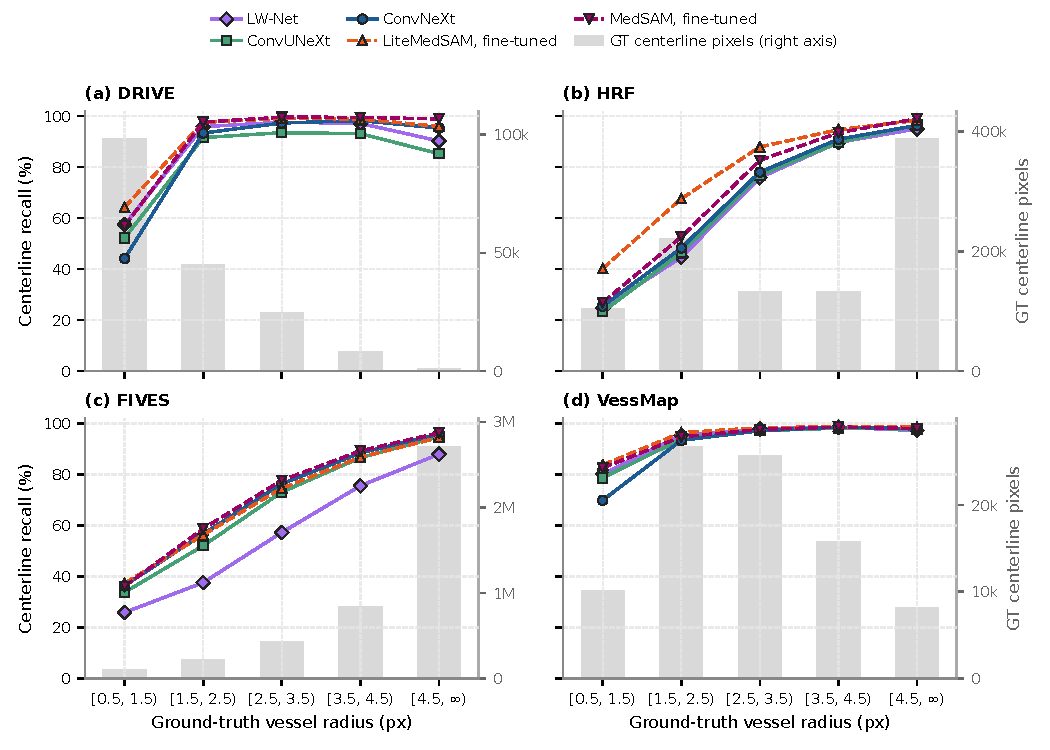
\includegraphics[width=\textwidth]{figures/fig01_recall_by_caliber.pdf}
\caption{Centerline recall by ground-truth vessel radius (means over the test images). The first bin, radius in $[0.5, 1.5)$~px, is $\thinrecall$. Grey bars (right axis, own scale per panel): ground-truth centerline pixels per bin, summed over the test images.}
\label{fig:recall_caliber}
\end{figure*}

A model can raise its $\thinrecall$ by over-segmenting, for example by predicting vessels that are not in the ground truth. Fig.~\ref{fig:thin_pr} therefore plots the centerline precision of thin vessels, $P_{\mathrm{thin}}$, which is computed on the thin centerline pixels of the prediction (Section~\ref{subsec:method_metrics}), so thin vessels that a model draws outside the ground truth lower it.

\begin{figure*}[tbp]
\centering
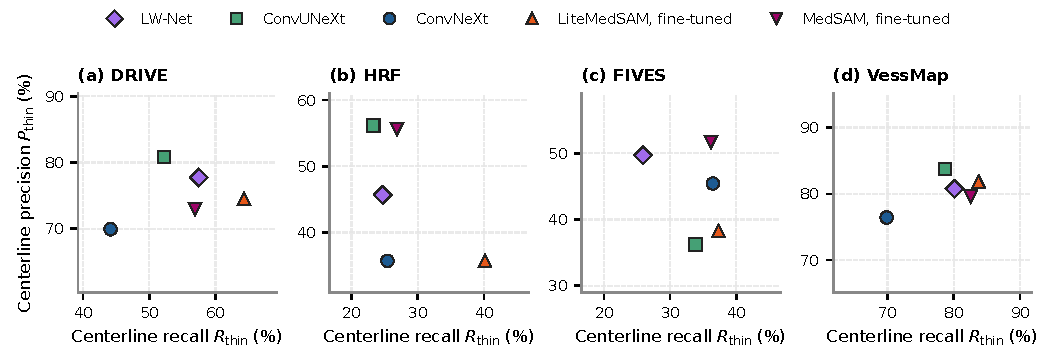
\includegraphics[width=\textwidth]{figures/fig02_thin_precision_recall.pdf}
\caption{Centerline precision against centerline recall of thin vessels, per dataset (means over the test images). Every panel spans the same width on both axes.}
\label{fig:thin_pr}
\end{figure*}

On HRF and FIVES, the $P_{\mathrm{thin}}$ of fine-tuned \medsam{} was not significantly lower than that of any CNN, and on FIVES it was the highest of the five models. On DRIVE and VessMap, it was significantly lower than that of \convunext{}, the best CNN, by 7.8 and 4.2 points, and on DRIVE also than that of \lwnet{}. The higher $\thinrecall$ of \litemedsam{} came with a lower $P_{\mathrm{thin}}$ than that of the best CNN on every dataset, significantly on DRIVE, HRF and FIVES. Table~\ref{tab:pvalues} gives the test of every pair of configurations.

\begin{figure*}[tbp]
\centering
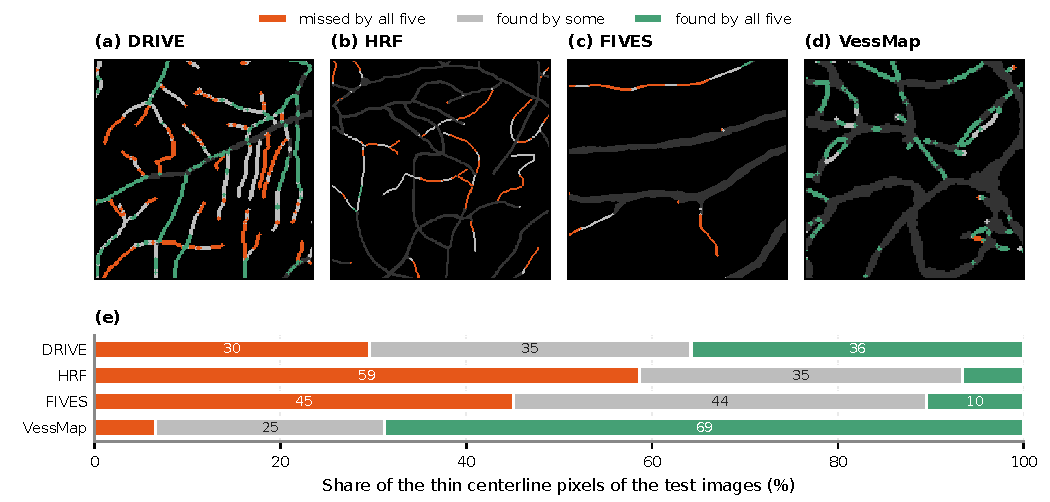
\includegraphics[width=\textwidth]{figures/fig07_thin_errors.pdf}
\caption{Ground-truth thin centerline pixels found by all five models of Table~\ref{tab:global_baseline}, by some or by
none (\medsam{} with the upscaled protocol). (a--d) The window of each test set with the most thin centerline pixels
(160, 320, 256 and 128~px), over the ground-truth vessels (dark grey on black). (e) Shares over all test images.}
\label{fig:thin_errors}
\end{figure*}

Fig.~\ref{fig:thin_errors} shows where the five models find and miss thin vessels. On every dataset, most thin
centerline pixels were found by all five models or missed by all five, so the models succeed and fail largely on the
same thin vessels. A missed thin centerline pixel is either close to a predicted vessel, within 2~px, when the model
drew the vessel slightly offset or narrower, or far from any predicted vessel, when the model did not draw it. On HRF
and FIVES, the largest share was missed by all five and most misses were far; on DRIVE and VessMap, more of the misses
were close, and a metric with a distance tolerance of 2~px would count them as found. The thin vessels that separate the models are a minority of the thin centerline, which
is consistent with the absence of a significant difference in $\thinrecall$ between fine-tuned \medsam{} and the best
CNN.

\subsection{Cost and the compact plain ViT}
\label{subsec:results_cost}

\begin{figure*}[tbp]
\centering
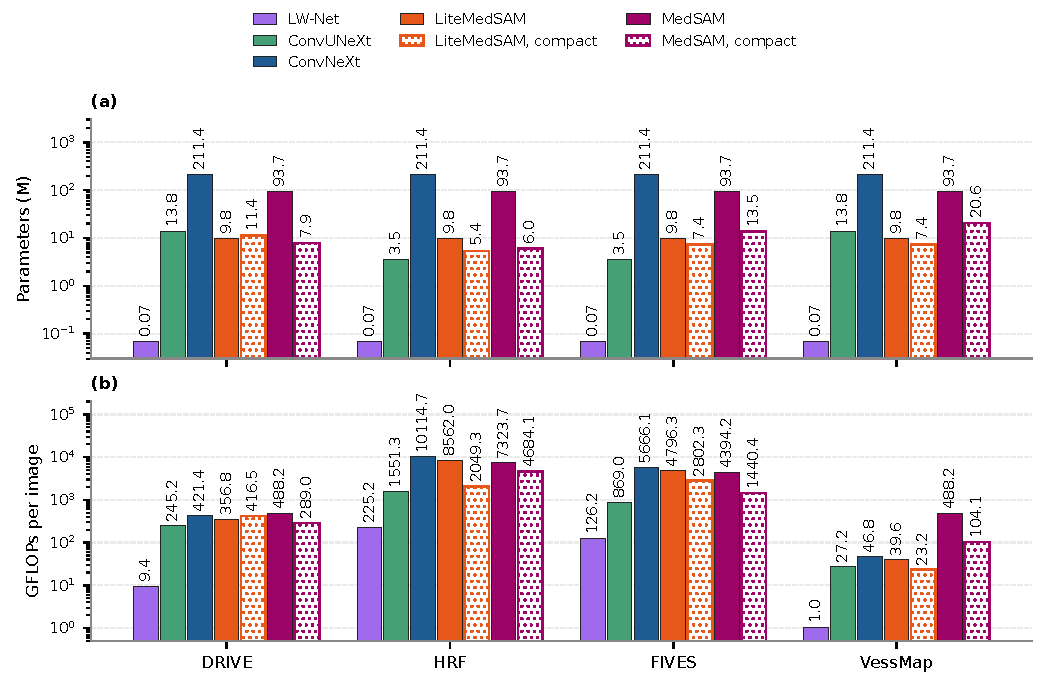
\includegraphics[width=\textwidth]{figures/fig03_cost.pdf}
\caption{Cost of each architecture: (a)~parameters and (b)~GFLOPs per test image, log scale. Fine-tuned and from-scratch runs share one bar.}
\label{fig:cost}
\end{figure*}

\begin{figure*}[tbp]
\centering
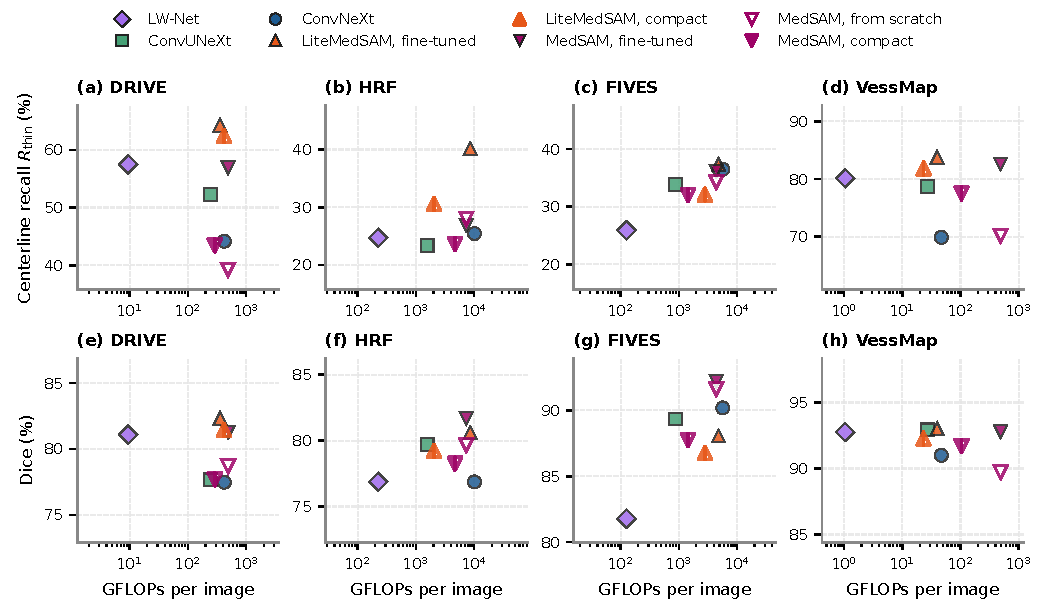
\includegraphics[width=\textwidth]{figures/fig04_compact_tradeoff.pdf}
\caption{$\thinrecall$ (a--d) and Dice (e--h) against GFLOPs per test image (log scale; means over the test images). Compact: \medsam{} and \litemedsam{} with a 256~px window and a searched size, trained from scratch. Within a row, every panel spans the same range width.}
\label{fig:compact_tradeoff}
\end{figure*}

Fig.~\ref{fig:cost} gives the parameters and the GFLOPs per test image of each architecture. \medsam{} had the second-largest parameter count, after \convnext{}, and the highest cost per image on DRIVE and VessMap, whose images are smaller than its 1024~px window and are upscaled to it. On the larger HRF and FIVES images, the models with 256~px windows need many more windows per image than \medsam{}, so \convnext{} and \litemedsam{} cost more per image than \medsam{}. The hybrid \litemedsam{}, in the second class by parameters, had the highest mean $\thinrecall$ on every dataset but a lower $P_{\mathrm{thin}}$ than the best CNN, significantly on three datasets (Section~\ref{subsec:results_thin}), and on HRF and FIVES it cost more per image than \medsam{}.

By parameter count, the models fall into three cost classes (Fig.~\ref{fig:cost}a): \medsam{} and \convnext{}; the compact models, \litemedsam{} and \convunext{}; and \lwnet{}. Models can be compared fairly within a class, unless the aim is the highest accuracy at any cost. The classes hold for parameters, not for GFLOPs per image on HRF and FIVES. The search for compact \litemedsam{}, which was not limited to models smaller than \litemedsam{}, returned models of the same order of size and cost as \litemedsam{}, and on DRIVE a slightly larger one (Table~\ref{tab:compact_models}).

Fine-tuned \medsam{}, whose $\thinrecall$ was not significantly different from that of the best CNN on any dataset, belongs to the most expensive class. Its compact version, in the second class, did not keep this performance (Fig.~\ref{fig:compact_tradeoff}): against the best CNN, its $\thinrecall$ was significantly lower on DRIVE and FIVES, and its $P_{\mathrm{thin}}$ and Dice were significantly lower on all four datasets (Table~\ref{tab:pvalues}). Its cost per image was within the range of the CNNs except on VessMap. Compact \medsam{} differs from fine-tuned \medsam{} in size, initialization, patch size, input window and, on DRIVE and VessMap, input scale, so this comparison does not separate them; Fig.~\ref{fig:pretraining} compares the same architectures with and without pre-training.

The search for compact \medsam{} selected finer patches than the 16~px of \medsam{}: 4~px, and 8~px on FIVES (Table~\ref{tab:patch_size}). With 16~px patches, its best validation Dice was 15.7\% on DRIVE and 14.0\% on HRF. Other hyperparameters varied between these trials, so Table~\ref{tab:patch_size} is not a controlled comparison of patch sizes.

\subsection{Pre-training and training difficulty}
\label{subsec:results_pretraining}

\begin{figure*}[tbp]
\centering
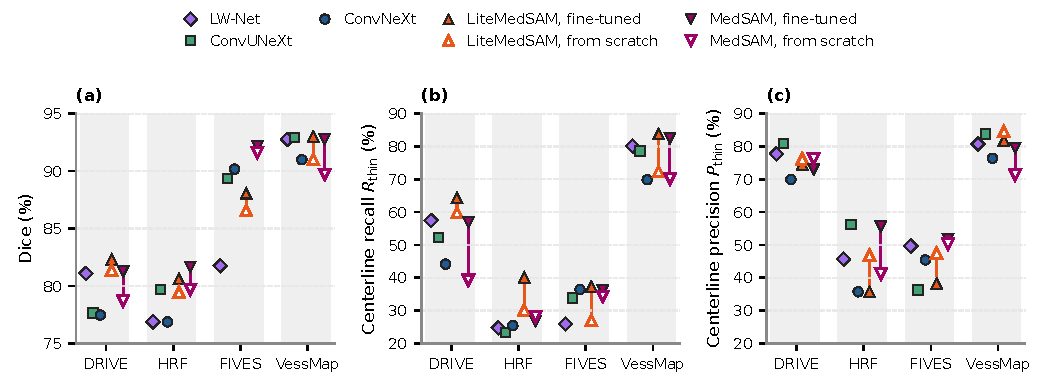
\includegraphics[width=\textwidth]{figures/fig05_pretraining.pdf}
\caption{Effect of pre-training: (a)~Dice, (b)~$\thinrecall$ and (c)~$P_{\mathrm{thin}}$ of the two transformer-based models fine-tuned (filled) and trained from scratch (hollow), next to the CNNs (means over the test images). Panels (b) and (c) share one vertical range.}
\label{fig:pretraining}
\end{figure*}

Fig.~\ref{fig:pretraining} compares \medsam{} and \litemedsam{} fine-tuned from their pre-trained weights with the same architectures trained from scratch, next to the three CNNs; Table~\ref{tab:pretraining_gain} in Appendix~\ref{app:results_detail} gives the gain from pre-training, fine-tuned minus from scratch.

\begin{figure*}[tbp]
\centering
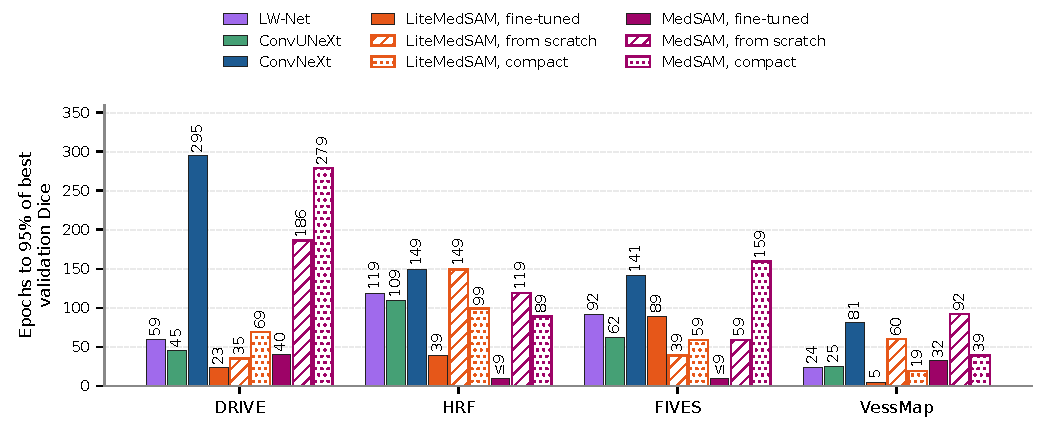
\includegraphics[width=\textwidth]{figures/fig06_convergence.pdf}
\caption{Epochs until the selected run first reached 95\% of its best validation Dice (validation every epoch or every 10 epochs; ``$\le$'': reached at the first validation). One run per configuration.}
\label{fig:convergence}
\end{figure*}

Pre-training raised the Dice of \medsam{} significantly on every dataset (Fig.~\ref{fig:pretraining}a; Table~\ref{tab:pretraining_gain}). Its effect on the $\thinrecall$ of \medsam{} depended on the dataset: it rose by 17.6 and 12.4 points on DRIVE and VessMap, much less on FIVES and not significantly on HRF. For the hybrid \litemedsam{}, pre-training raised $\thinrecall$ significantly on every dataset and Dice by less. Trained from scratch, \litemedsam{} had a higher $P_{\mathrm{thin}}$, significantly on HRF and FIVES. Without pre-training, the $\thinrecall$ of \medsam{} was significantly lower than that of the best CNN on DRIVE, FIVES and VessMap, and not on HRF.

Without pre-training, \medsam{} also needed more epochs to reach 95\% of its best validation Dice on every dataset (Fig.~\ref{fig:convergence}), and so did compact \medsam{}. For \litemedsam{} the pattern was mixed: from scratch it needed more epochs on DRIVE, HRF and VessMap and fewer on FIVES. Each of these values comes from one training run.

Table~\ref{tab:medsam_vs_cnn} compares fine-tuned \medsam{} with the best CNN of each metric and dataset. On HRF and FIVES, its Dice was significantly higher, by 2.0 points, with no significant difference in either thin-vessel metric (Tables~\ref{tab:medsam_vs_cnn} and~\ref{tab:pvalues}); on DRIVE and VessMap, its Dice was not significantly different. It also reached 95\% of its best validation Dice in fewer epochs than the CNN with the highest Dice on DRIVE, HRF and FIVES.

For \medsam{}, the Dice gain from pre-training was smallest on FIVES, the dataset with the most training images, with no order by number of images among the other three. For \litemedsam{}, the gains in Dice and $\thinrecall$ instead grew from DRIVE to HRF to VessMap, in the order of their number of training images, and were not smallest on FIVES (Table~\ref{tab:pretraining_gain}). The four datasets also differ in resolution, imaging domain and the upscaling of \medsam{}, so the number of training images is not isolated.

% Generated by paper/figures_tables/tab03_medsam_vs_cnn.py -- do not edit by hand.
% Source: results/per_image_metrics.csv (MedSAM DRIVE/VessMap upscaled protocol); results/convergence.csv.
\begin{table*}[tbp]
\caption{Fine-tuned \medsam{} against the best CNN of each metric and dataset (L: \lwnet{}, U: \convunext{}, N:
\convnext{}); $\Delta$: \medsam{} minus the best CNN. Bold: best; $^{*}$: significant. Epochs: of \medsam{} and of the
CNN with the highest Dice
(bold: fewer; ``$\le$'': reached at the first validation).}
\label{tab:medsam_vs_cnn}
\begin{ruledtabular}
\begin{tabular}{lcccccccc}
 & \multicolumn{3}{c}{Dice} & \multicolumn{3}{c}{$\thinrecall$} & \multicolumn{2}{c}{Epochs} \\
\cmidrule(lr){2-4} \cmidrule(lr){5-7} \cmidrule(lr){8-9}
Dataset & \medsam{} & Best CNN & $\Delta$ & \medsam{} & Best CNN & $\Delta$ & \medsam{} & CNN \\
\midrule
\shortstack{DRIVE\\($n=20$)} & {\boldmath$81.3 \pm 1.3$} & $81.1 \pm 2.4$\textsuperscript{L} & $+0.2$ & $56.9 \pm 11.8$ & {\boldmath$57.5 \pm 12.1$}\textsuperscript{L} & $-0.6$ & \textbf{40} & 59 \\
\shortstack{HRF\\($n=14$)} & {\boldmath$81.7 \pm 4.5$} & $79.7 \pm 5.1$\textsuperscript{U} & $+2.0^{*}$ & {\boldmath$26.9 \pm 17.2$} & $25.4 \pm 13.5$\textsuperscript{N} & $+1.5$ & \textbf{$\le$9} & 109 \\
\shortstack{FIVES\\($n=200$)} & {\boldmath$92.2 \pm 8.5$} & $90.2 \pm 8.5$\textsuperscript{N} & $+2.0^{*}$ & $36.2 \pm 11.9$ & {\boldmath$36.5 \pm 12.2$}\textsuperscript{N} & $-0.3$ & \textbf{$\le$9} & 141 \\
\shortstack{VessMap\\($n=30$)} & $92.8 \pm 2.1$ & {\boldmath$92.9 \pm 2.1$}\textsuperscript{U} & $-0.1$ & {\boldmath$82.6 \pm 14.1$} & $80.1 \pm 12.2$\textsuperscript{L} & $+2.5$ & 32 & \textbf{25} \\
\end{tabular}
\end{ruledtabular}
\end{table*}


% Generated by paper/figures_tables/tab02_padding_protocol.py -- do not edit by hand.
% Source: results/per_image_metrics.csv (native = padded and upscaled protocols); GFLOPs per window from
% results/cost.csv; windows per image from MONAI's grid.
\begin{table*}[tbp]
\caption{The same \medsam{} checkpoints evaluated with the padded and the upscaled protocol; $\Delta$: upscaled minus
padded. Bold: best; $^{*}$: significant. $P_{\mathrm{thin}}$, VessMap, from scratch, padded: mean over 29 images (one image without predicted thin vessels).}
\label{tab:padding}
\begin{ruledtabular}
\begin{tabular}{llcccccc}
 & & \multicolumn{3}{c}{DRIVE ($n=20$)} & \multicolumn{3}{c}{VessMap ($n=30$)} \\
\cmidrule(lr){3-5} \cmidrule(lr){6-8}
\medsam{} & Metric & Padded & Upscaled & $\Delta$ & Padded & Upscaled & $\Delta$ \\
\midrule
\multirow{3}{*}{Fine-tuned} & Dice & $75.2 \pm 1.8$ & {\boldmath$81.3 \pm 1.3$} & $+6.1^{*}$ & $78.7 \pm 7.5$ & {\boldmath$92.8 \pm 2.1$} & $+14.1^{*}$ \\
 & $\thinrecall$ & $39.0 \pm 10.9$ & {\boldmath$56.9 \pm 11.8$} & $+17.9^{*}$ & $41.3 \pm 12.7$ & {\boldmath$82.6 \pm 14.1$} & $+41.3^{*}$ \\
 & $P_{\mathrm{thin}}$ & $58.8 \pm 7.9$ & {\boldmath$73.0 \pm 6.1$} & $+14.2^{*}$ & $76.8 \pm 13.2$ & {\boldmath$79.6 \pm 14.8$} & $+2.8$ \\
\midrule
\multirow{3}{*}{From scratch} & Dice & $65.7 \pm 3.0$ & {\boldmath$78.7 \pm 1.6$} & $+13.0^{*}$ & $68.2 \pm 6.4$ & {\boldmath$89.7 \pm 3.7$} & $+21.5^{*}$ \\
 & $\thinrecall$ & $25.3 \pm 8.0$ & {\boldmath$39.3 \pm 11.2$} & $+14.0^{*}$ & $43.6 \pm 19.2$ & {\boldmath$70.2 \pm 20.9$} & $+26.6^{*}$ \\
 & $P_{\mathrm{thin}}$ & $56.5 \pm 8.8$ & {\boldmath$76.2 \pm 7.0$} & $+19.7^{*}$ & $57.5 \pm 21.3$ & {\boldmath$71.4 \pm 14.1$} & $+13.9^{*}$ \\
\end{tabular}
\end{ruledtabular}
\end{table*}


\subsection{Inference protocol of MedSAM: padding versus upscaling}
\label{subsec:results_padding}

On DRIVE and VessMap, both protocols of Section~\ref{subsec:method_metrics} run one 1024~px window per image and have the same cost. The comparison is therefore not about a cheaper way to run \medsam{}: with the same checkpoints, padding makes each vessel span fewer input pixels than upscaling does.

The padded protocol gave a significantly lower Dice and $\thinrecall$ than the upscaled protocol for fine-tuned \medsam{} and \medsam{} trained from scratch on both datasets (Table~\ref{tab:padding}). For fine-tuned \medsam{}, $\thinrecall$ fell by 17.9 points on DRIVE and 41.3 points on VessMap, below the range of the CNNs on both datasets.

\subsection{Discussion}
\label{subsec:discussion}

The thin-vessel results of fine-tuned \medsam{} (Section~\ref{subsec:results_thin}) do not support the expectation that a plain ViT misses thin vessels, at least for \medsam{}, pre-trained on medical images~\cite{ma2024segment}, evaluated with the upscaled protocol.

The results bear on the argument that a 16~px token dilutes thin vessels (Section~\ref{sec:related_work}) in two ways, neither of which isolates it. On DRIVE and VessMap, \medsam{} saw the images upscaled, so a 16~px patch covered a square of about 9 and 4 native pixels on a side (Section~\ref{subsec:method_training}). With the native image padded into the window, the same checkpoints lost much of their $\thinrecall$ (Table~\ref{tab:padding}). This is consistent with the extent of a token in native pixels mattering for thin vessels, but padding also changes the scale at which the model sees the image relative to training, and the two explanations cannot be separated here. On HRF and FIVES, where \medsam{} tokenized native pixels in 16~px patches, its $\thinrecall$ was also within or above the range of the CNNs, although $\thinrecall$ was low for every model on these two datasets.

The hybrid \litemedsam{} had the highest mean $\thinrecall$ on every dataset but a lower $P_{\mathrm{thin}}$ than the best CNN on all four, so its higher recall is not by itself evidence of a better segmentation of thin vessels.

Our results on the compact plain ViT are limited in two ways. First, compact \medsam{} differs from fine-tuned \medsam{} in several properties at once (Section~\ref{subsec:results_cost}), so the results cannot say which of these accounts for its loss of thin-vessel performance; they show only that the plain ViT obtained its $\thinrecall$ as a model of the most expensive class and that a compact version in the second class did not keep it (Section~\ref{subsec:results_cost}). Second, the search selected one architecture per dataset by validation Dice and was not designed to study model size or patch size. Its preference for 4 or 8~px patches over 16~px patches on every dataset is therefore only consistent with the argument that a 16~px token dilutes thin vessels, for a plain ViT trained from scratch on a 256~px window. A study that varies the size of the plain ViT in a controlled way, including compact versions smaller than those selected here, could show where its thin-vessel performance is lost.

Our finding on thin vessels holds for the pre-trained \medsam{} only: trained from scratch, it fell below the best CNN in $\thinrecall$ on three datasets (Section~\ref{subsec:results_pretraining}). This gain from pre-training is measured against our from-scratch recipe, which used the learning rates searched for fine-tuning, batch sizes of 1 to 4 and no warm-up; a recipe designed for training a ViT from scratch could reduce it. Trained from scratch, the hybrid detected fewer thin vessels on every dataset and, on HRF and FIVES, a larger share of the thin vessels it drew was in the ground truth, which is consistent with a more conservative segmentation of thin vessels.

Our data answer only in part how the gain from pre-training depends on the number of training images, and the answer differs between the two models. For \medsam{}, the Dice gain was smallest on FIVES, the dataset with the most training images, which is consistent with pre-training adding less when more training images are available; its $\thinrecall$ gain was large on the two datasets it saw upscaled and small or absent on the other two, an order that does not follow the number of training images. For \litemedsam{}, the gains grew with the number of training images over the three smaller datasets and were not smallest on FIVES, which does not fit that reading. With four datasets that also differ in resolution, domain and upscaling, these are orders over four points, not estimates of how the gain depends on the number of images.

The advantage of the pre-trained plain ViT over the CNNs trained from scratch was small: a higher Dice on HRF and FIVES without a significant difference in either thin-vessel metric, and none on DRIVE and VessMap, where its $P_{\mathrm{thin}}$ was significantly lower than that of the best CNN.

We did not measure how finely each dataset was annotated, a possible factor in the thin-vessel results. Thin vessels hold a much larger share of the ground-truth centerline on DRIVE than on FIVES (Section~\ref{subsec:results_overall}). Part of this difference comes from resolution, since a vessel of a given width spans more pixels in the larger HRF and FIVES images. Part may come from annotation detail, if DRIVE was annotated down to finer vessels than FIVES, a dataset with many more images. A thin vessel that a model detects but the annotation omits lowers its $P_{\mathrm{thin}}$, which may contribute to the lower $P_{\mathrm{thin}}$ of every model on HRF and FIVES than on DRIVE and VessMap (Fig.~\ref{fig:thin_pr}).

We observed the effect of padding for one model on two datasets, but it is a methodological point for evaluating a plain ViT on images smaller than its input window: on DRIVE and VessMap, whether fine-tuned \medsam{} had a $\thinrecall$ within the range of the CNNs depended on the inference protocol (Table~\ref{tab:padding}). A study that evaluates such a model on small images should therefore evaluate it at the scale used in training and state that scale.

Six limitations concern how the models were trained, selected and measured. Each configuration was trained once, with one random seed, so the variation between training runs is unknown. For Little W-Net, the published 95\% confidence interval of the mean DRIVE Dice over five runs is $\pm 0.11$ points~\cite{galdran2020littlewnetcouldstateoftheart}, but ours was not measured. The Wilcoxon tests take the test images as the sample, so they generalize over test images, not over training runs; on HRF, with 14 test images, they detect only large or very consistent differences. On HRF, FIVES and VessMap, checkpoint selection, early stopping and the hyperparameter search used the test images (Section~\ref{subsec:method_problem_data}). The comparison across architectures pairs CNNs trained from scratch with fine-tuned transformer-based models, so it mixes architecture and initialization: ImageNet weights exist for the ConvNeXt-Large encoder~\cite{liu2022convnet}, but they come from natural images, so we did not use them, and we found no public CNN pre-trained on a medical image collection comparable to that of \medsam{}. \medsam{} saw DRIVE and VessMap upscaled, and on every dataset its window covered 16 times the area of the other models' windows; the CNNs were not trained at this scale or window, so the comparison does not separate the architecture from the input scale and window. Finally, we measured cost as parameters and GFLOPs, not as latency or throughput.

\section{Conclusion}
\label{sec:conclusion}

We compared a plain ViT (\medsam{}), a hybrid (\litemedsam{}) and three CNNs on the thin vessels of three retinal datasets, DRIVE, HRF and FIVES, with VessMap as a check in a second imaging domain.

Fine-tuned from its pre-trained weights and evaluated with the upscaled protocol, \medsam{} had an $\thinrecall$ not significantly different from that of the best CNN on all four datasets, and a significantly lower $P_{\mathrm{thin}}$ on DRIVE and VessMap. For \medsam{} in these conditions, the results on these datasets do not support the expectation that a plain ViT misses thin vessels.

\medsam{} reached this as a model of the most expensive class by parameter count. A compact plain ViT trained from scratch, in the class of \litemedsam{} and \convunext{}, did not keep this performance: against the best CNN, its $\thinrecall$ was significantly lower on DRIVE and FIVES, and its $P_{\mathrm{thin}}$ and Dice on all four datasets. The hybrid \litemedsam{}, in the same class, had the highest mean $\thinrecall$ on every dataset, but a lower $P_{\mathrm{thin}}$ than the best CNN, significantly on three datasets. Where cost matters, the smallest CNN remains a candidate on small images: \lwnet{}, with 0.07~M parameters, had a Dice and an $\thinrecall$ not significantly different from those of fine-tuned \medsam{} on DRIVE and VessMap, and on DRIVE a significantly higher $P_{\mathrm{thin}}$ (Table~\ref{tab:pvalues}), at a small fraction of its cost per image (Fig.~\ref{fig:cost}).

Pre-training raised the Dice of \medsam{} significantly on every dataset; without it, \medsam{} fell significantly below the best CNN in $\thinrecall$ on three datasets. The hybrid \litemedsam{} depended less on pre-training for Dice than for $\thinrecall$. The Dice gain of \medsam{} was smallest on FIVES, the dataset with the most training images, while the gains of \litemedsam{} did not follow this order; four datasets that also differ in resolution, domain and upscaling cannot isolate the number of images. On HRF and FIVES, fine-tuned \medsam{} had a significantly higher Dice than the best CNN, with no significant loss in $\thinrecall$ or $P_{\mathrm{thin}}$.

On DRIVE and VessMap, whose images are smaller than the window of \medsam{}, padding the images instead of upscaling them to the window lowered its $\thinrecall$ below the range of the CNNs at the same cost. For \medsam{} on these two datasets, the thin-vessel results depend on evaluating it at the scale it was trained on, and a study of a plain ViT on images smaller than its window should state that scale.

Each configuration was trained once, so the tests generalize over test images and not over training runs, and the comparison across architectures mixes initializations and input scales. Future work should repeat the comparison over several training runs and on more datasets, train the CNNs at the input scale and window of \medsam{}, train the plain ViT from scratch with a recipe designed for it, test the patch size of a plain ViT with the other hyperparameters fixed, and measure inference latency.

\section*{Code availability}
The code for training, the hyperparameter search and the figures is available at \url{https://github.com/CarlosFontaneli/thin-vessel-sam-cnn}.

\clearpage
\appendix

\section{Training details}
\label{app:training}

\subsection{Data preparation, sampling and augmentation}
In 106 training masks and 5 test masks of FIVES, pixels along the image border were labelled as vessel; we set a 2~px border of these masks to background. Each training sample was taken from one training image with random horizontal and vertical flips (probability 0.5 each) and a random rotation between $-30^\circ$ and $30^\circ$. The sample was then cropped at a random position to the model's input size: 256~px for the CNNs, \litemedsam{} and the compact models, and 1024~px for \medsam{}. Images smaller than the input size, which is the case for DRIVE ($565 \times 584$~px) and VessMap ($256 \times 256$~px) with \medsam{}, were upscaled to it instead, with bilinear interpolation for the image and nearest-exact interpolation for the mask, which keeps the mask binary.

\subsection{Loss function}
All models were trained with the soft Dice loss with squared terms in the denominator~\cite{milletari2016vnet},
\begin{equation}
    \mathcal{L}_{\text{Dice}}(Y, \hat{Y}) = 1 - \frac{2 \sum_{i,j} Y_{i,j} \hat{Y}_{i,j} + \epsilon}{\sum_{i,j} Y_{i,j}^2 + \sum_{i,j} \hat{Y}_{i,j}^2 + \epsilon},
    \label{eq:dice_loss}
\end{equation}
where $\hat{Y}$ is the sigmoid output and $\epsilon = 10^{-5}$, computed for each image and averaged over the batch. \lwnet{} produces a coarse and a refined segmentation; its loss is the sum of Eq.~\eqref{eq:dice_loss} for the two outputs.

\subsection{Hyperparameter search}
Table~\ref{tab:search_space} lists the search of each configuration and dataset, and Table~\ref{tab:compact_models} the architectures of the compact models. Every run used AdamW with a cosine learning-rate schedule~\cite{loshchilov2017sgdr} over at most 1000 epochs.

We ran the searches with Optuna~\cite{akiba2019optuna} (version 4.7.0), using its tree-structured Parzen estimator sampler~\cite{bergstra2011algorithms} and median pruning on the validation Dice. For the compact models the search also covered the architecture: the patch size, embedding dimension, depth, number of heads, MLP ratio and attention window of compact \medsam{}, and the per-stage widths and depths of compact \litemedsam{}. It selected one compact model per dataset (Table~\ref{tab:compact_models}); Table~\ref{tab:patch_size} gives the best validation Dice the search reached with each patch size. Fine-tuned and from-scratch runs of a transformer-based model share the architecture and therefore the cost. In total, the 36 searches ran 3,602 trials in 2,093 GPU hours (the sum of the trial durations, one GPU per trial). The CNNs were trained on an NVIDIA RTX 3090 GPU and the transformer-based models on NVIDIA RTX PRO 5000 (48~GB) and RTX PRO 4000 (24~GB) GPUs.

For the CNNs, the search covered one architecture parameter each (Table~\ref{tab:search_space}). For \lwnet{} (first-level width) and \convunext{} (base width), it sets the size of the model; it was searched on DRIVE, FIVES and VessMap and fixed on HRF. The selected \lwnet{} has a first width of 8 on every dataset (0.07~M parameters), and the selected \convunext{} a base width of 64 on DRIVE and VessMap (13.8~M) and 32 on HRF and FIVES (3.5~M). The stochastic-depth rate of \convnext{} does not change its size (211.4~M).

Validation runs the sliding-window inference over the full validation images. To reduce the training time spent on it, we validated every 10 epochs on HRF, for every compact model, and for the transformer-based models on FIVES; we validated every epoch for the other runs on DRIVE and VessMap and for \lwnet{} and \convunext{} on FIVES. The early-stopping patience was 5 validations when validating every 10 epochs and 50 when validating every epoch, so training stopped after 50 epochs without improvement in both cases. The interval of 10 epochs was introduced while the FIVES searches of \convnext{} and fine-tuned \litemedsam{} were running: their first 2 and 15 trials, which include the selected runs, were validated every epoch, and the later ones every 10 epochs.

For \medsam{} on DRIVE and VessMap, validation used the padded protocol of Section~\ref{subsec:method_metrics}, the native image padded to the 1024~px window, while every test result of \medsam{} uses the upscaled protocol. The checkpoints of these runs were therefore selected, and their epochs in Fig.~\ref{fig:convergence} measured, under the padded protocol, which cannot be changed without retraining.

Within a trial we kept the checkpoint with the highest validation Dice, and for each configuration we report the trial with the highest validation Dice among the trials that finished.

% Generated by paper/figures_tables/tabA1_search_space.py -- do not edit by hand.
% Source: results/search_trials.csv (exported from the Optuna studies, trial configurations and train.log by
% scripts/analyse.py) and the released configurations under configs/.
\begin{table*}[tbp]
\caption{Hyperparameter search (100 trials; 101 where one failed). Learning rate and weight decay: log-uniform in the
ranges shown. CNN architecture parameter: \lwnet{}, width of the first of its three levels (doubled at each level);
\convunext{}, base width; \convnext{}, stochastic-depth rate. Val.: validation interval of the selected run
(epochs); Trials: finished trials; GPU~h: sum of the trial durations.}
\label{tab:search_space}
\footnotesize
\begin{ruledtabular}
\begin{tabular}{llcccccrr}
Configuration & Dataset & Learning rate & Weight decay & Batch size & Architecture & Val. & Trials & GPU~h \\
\midrule
\multirow{4}{*}{\lwnet{}} & DRIVE & $10^{-6}$--$10^{-1}$ & $10^{-6}$--$10^{-1}$ & 2, 4, 8 & first width 8, 16, 32 & 1 & 100 & 13.0 \\
 & HRF & $10^{-6}$--$10^{-1}$ & $10^{-6}$--$10^{-1}$ & 2, 4, 8, 16 & -- & 10 & 100 & 34.0 \\
 & FIVES & $10^{-6}$--$10^{-1}$ & $10^{-6}$--$10^{-1}$ & 2, 4, 8, 16, 32, 64 & first width 8, 16, 32 & 1 & 100 & 108.6 \\
 & VessMap & $10^{-5}$--$10^{-2}$ & $10^{-5}$--$10^{-1}$ & 2, 4, 8, 16, 32 & first width 8, 16, 32 & 1 & 100 & 1.2 \\
\midrule
\multirow{4}{*}{\convunext{}} & DRIVE & $10^{-6}$--$10^{-2}$ & $10^{-6}$--$10^{-1}$ & 2, 4, 8 & base width 16, 32, 64 & 1 & 100 & 13.4 \\
 & HRF & $10^{-6}$--$10^{-2}$ & $10^{-6}$--$10^{-1}$ & 2, 4, 8, 16 & -- & 10 & 100 & 25.1 \\
 & FIVES & $10^{-6}$--$10^{-2}$ & $10^{-6}$--$10^{-1}$ & 2, 4, 8, 16, 32, 64 & base width 16, 32, 64 & 1 & 100 & 292.6 \\
 & VessMap & $10^{-5}$--$10^{-2}$ & $10^{-5}$--$10^{-1}$ & 2, 4, 8, 16, 32 & base width 16, 32, 64 & 1 & 100 & 2.5 \\
\midrule
\multirow{4}{*}{\convnext{}} & DRIVE & $10^{-6}$--$10^{-2}$ & $10^{-6}$--$10^{-1}$ & 2, 4, 8 & drop-path rate 0--0.5 & 1 & 100 & 15.1 \\
 & HRF & $10^{-6}$--$10^{-2}$ & $10^{-6}$--$10^{-1}$ & 2, 4, 8, 16 & drop-path rate 0--0.5 & 10 & 100 & 40.2 \\
 & FIVES & $10^{-6}$--$10^{-2}$ & $10^{-6}$--$10^{-1}$ & 2, 4, 8, 16, 32 & drop-path rate 0--0.5 & 1 & 100 & 210.5 \\
 & VessMap & $10^{-5}$--$10^{-2}$ & $10^{-5}$--$10^{-1}$ & 2, 4, 8, 16, 32 & drop-path rate 0--0.5 & 1 & 100 & 31.5 \\
\midrule
\multirow{4}{*}{\litemedsam{}, fine-tuned} & DRIVE & $10^{-6}$--$10^{-2}$ & $10^{-6}$--$10^{-1}$ & 2, 4, 8 & -- & 1 & 100 & 7.6 \\
 & HRF & $10^{-6}$--$10^{-2}$ & $10^{-6}$--$10^{-1}$ & 4, 8 & -- & 10 & 100 & 7.0 \\
 & FIVES & $10^{-6}$--$10^{-2}$ & $10^{-6}$--$10^{-1}$ & 8, 16 & -- & 1 & 100 & 117.3 \\
 & VessMap & $10^{-5}$--$10^{-2}$ & $10^{-5}$--$10^{-1}$ & 2, 4, 8 & -- & 1 & 100 & 20.9 \\
\midrule
\multirow{4}{*}{\litemedsam{}, from scratch} & DRIVE & $10^{-6}$--$10^{-2}$ & $10^{-6}$--$10^{-1}$ & 1, 2, 4 & -- & 1 & 100 & 17.4 \\
 & HRF & $10^{-6}$--$10^{-2}$ & $10^{-6}$--$10^{-1}$ & 4, 8 & -- & 10 & 100 & 13.6 \\
 & FIVES & $10^{-6}$--$10^{-2}$ & $10^{-6}$--$10^{-1}$ & 4, 8 & -- & 10 & 100 & 138.1 \\
 & VessMap & $10^{-5}$--$10^{-2}$ & $10^{-5}$--$10^{-1}$ & 1, 2, 4 & -- & 1 & 100 & 9.0 \\
\midrule
\multirow{4}{*}{\litemedsam{}, compact} & DRIVE & $10^{-6}$--$10^{-2}$ & $10^{-6}$--$10^{-1}$ & 8, 16, 32 & Table~\ref{tab:compact_models} & 10 & 100 & 1.7 \\
 & HRF & $10^{-6}$--$10^{-2}$ & $10^{-6}$--$10^{-1}$ & 8, 16, 32 & Table~\ref{tab:compact_models} & 10 & 100 & 11.6 \\
 & FIVES & $10^{-6}$--$10^{-2}$ & $10^{-6}$--$10^{-1}$ & 8, 16, 32 & Table~\ref{tab:compact_models} & 10 & 101 & 107.3 \\
 & VessMap & $10^{-5}$--$10^{-2}$ & $10^{-5}$--$10^{-1}$ & 8, 16, 32 & Table~\ref{tab:compact_models} & 10 & 100 & 17.2 \\
\midrule
\multirow{4}{*}{\medsam{}, fine-tuned} & DRIVE & $10^{-7}$--$10^{-3}$ & $10^{-6}$--$10^{-1}$ & 2 & -- & 1 & 100 & 9.9 \\
 & HRF & $10^{-7}$--$10^{-3}$ & $10^{-6}$--$10^{-1}$ & 2, 4 & -- & 10 & 100 & 15.0 \\
 & FIVES & $10^{-7}$--$10^{-3}$ & $10^{-6}$--$10^{-1}$ & 2, 4 & -- & 10 & 100 & 277.1 \\
 & VessMap & $10^{-5}$--$10^{-2}$ & $10^{-5}$--$10^{-1}$ & 2 & -- & 1 & 100 & 21.1 \\
\midrule
\multirow{4}{*}{\medsam{}, from scratch} & DRIVE & $10^{-7}$--$10^{-3}$ & $10^{-6}$--$10^{-1}$ & 1 & -- & 1 & 100 & 28.6 \\
 & HRF & $10^{-7}$--$10^{-3}$ & $10^{-6}$--$10^{-1}$ & 1, 2, 4 & -- & 10 & 100 & 20.8 \\
 & FIVES & $10^{-7}$--$10^{-3}$ & $10^{-6}$--$10^{-1}$ & 1, 2, 4 & -- & 10 & 100 & 345.2 \\
 & VessMap & $10^{-5}$--$10^{-2}$ & $10^{-5}$--$10^{-1}$ & 1 & -- & 1 & 100 & 26.3 \\
\midrule
\multirow{4}{*}{\medsam{}, compact} & DRIVE & $10^{-7}$--$10^{-3}$ & $10^{-6}$--$10^{-1}$ & 4, 8, 16 & Table~\ref{tab:compact_models} & 10 & 101 & 0.9 \\
 & HRF & $10^{-7}$--$10^{-3}$ & $10^{-6}$--$10^{-1}$ & 4, 8, 16 & Table~\ref{tab:compact_models} & 10 & 100 & 7.6 \\
 & FIVES & $10^{-7}$--$10^{-3}$ & $10^{-6}$--$10^{-1}$ & 4, 8, 16 & Table~\ref{tab:compact_models} & 10 & 100 & 66.5 \\
 & VessMap & $10^{-5}$--$10^{-2}$ & $10^{-5}$--$10^{-1}$ & 4, 8, 16 & Table~\ref{tab:compact_models} & 10 & 100 & 17.7 \\
\end{tabular}
\end{ruledtabular}
\end{table*}

% Generated by paper/figures_tables/tabA2_compact_models.py -- do not edit by hand.
% Source: configs/ (selected trials and search spaces); results/cost.csv (parameters).
\begin{table*}[tbp]
\caption{Selected compact models and the original \medsam{} and \litemedsam{} (same architecture fine-tuned and
from scratch). Input, Patch: px; Tokens: grid of one window; Emb.: embedding dimension; MLP: ratio of the hidden
width of the feed-forward (MLP) block to the embedding dimension; Window:
attention window; Params: M; \litemedsam{}: per stage. Searched for compact \medsam{}: patch size
1, 2, 4, 8, 16
(1, 4, 8, 16 on DRIVE), embedding dimension 128, 256, 384, depth 4, 6, 8, heads 4, 8, MLP
ratio 2, 4, 6, attention window 7, 14; for compact \litemedsam{}: embedding dimensions
(32,64,80,160) or (64,128,160,320), depths (1,1,3,1) or (2,2,6,2), and on DRIVE only heads (1,2,2,5) or (2,4,5,10), attention windows
(7,7,7,7) or (7,7,14,7) and MLP ratio 2, 4, 6. Dice, $\thinrecall$,
$P_{\mathrm{thin}}$: compact
models (originals in Table~\ref{tab:pretraining_gain}).}
\label{tab:compact_models}
\scriptsize
\begin{ruledtabular}
\begin{tabular}{llccccccccrccc}
Model & Version & Input & Patch & Tokens & Emb. & Depth & Heads & MLP & Window & Params & Dice & $\thinrecall$ &
$P_{\mathrm{thin}}$ \\
\midrule
\multirow{5}{*}{\medsam{}} & original & 1024 & 16 & $64\times64$ & 768 & 12 & 12 & 4 & 14 & 93.7 & \multicolumn{3}{c}{Table~\ref{tab:pretraining_gain}} \\
 & compact, DRIVE & 256 & 4 & $64\times64$ & 256 & 4 & 8 & 2 & 14 & 7.9 & $77.7{\pm}2.5$ & $43.4{\pm}13.5$ & $69.3{\pm}8.3$ \\
 & compact, HRF & 256 & 4 & $64\times64$ & 128 & 6 & 4 & 2 & 14 & 6.0 & $78.3{\pm}5.9$ & $23.7{\pm}15.3$ & $43.3{\pm}11.6$ \\
 & compact, FIVES & 256 & 8 & $32\times32$ & 256 & 8 & 8 & 6 & 7 & 13.5 & $87.8{\pm}9.0$ & $32.0{\pm}11.3$ & $41.9{\pm}10.7$ \\
 & compact, VessMap & 256 & 4 & $64\times64$ & 384 & 6 & 4 & 6 & 7 & 20.6 & $91.7{\pm}2.8$ & $77.5{\pm}18.2$ & $74.5{\pm}14.5$ \\
\midrule
\multirow{5}{*}{\litemedsam{}} & original & 256 & -- & -- & 64,128,160,320 & 2,2,6,2 & 2,4,5,10 & 4 & 7,7,14,7 & 9.8 & \multicolumn{3}{c}{Table~\ref{tab:pretraining_gain}} \\
 & compact, DRIVE & 256 & -- & -- & 64,128,160,320 & 2,2,6,2 & 2,4,5,10 & 6 & 7,7,7,7 & 11.4 & $81.4{\pm}2.0$ & $62.4{\pm}12.1$ & $72.9{\pm}5.7$ \\
 & compact, HRF & 256 & -- & -- & 32,64,80,160 & 1,1,3,1 & 2,4,5,10 & 4 & 7,7,14,7 & 5.4 & $79.2{\pm}5.7$ & $30.5{\pm}13.9$ & $41.2{\pm}11.9$ \\
 & compact, FIVES & 256 & -- & -- & 64,128,160,320 & 1,1,3,1 & 2,4,5,10 & 4 & 7,7,14,7 & 7.4 & $86.7{\pm}10.8$ & $32.1{\pm}10.7$ & $41.2{\pm}12.1$ \\
 & compact, VessMap & 256 & -- & -- & 64,128,160,320 & 1,1,3,1 & 2,4,5,10 & 4 & 7,7,14,7 & 7.4 & $92.3{\pm}1.9$ & $81.8{\pm}11.5$ & $75.7{\pm}15.6$ \\
\end{tabular}
\end{ruledtabular}
\end{table*}

% Generated by paper/figures_tables/tabA3_patch_size.py -- do not edit by hand.
% Source: results/search_trials.csv (compact-MedSAM studies).
\begin{table}[tbp]
\caption{Patch size in the search of compact \medsam{}: trials that reached a validation (Tr.) and their best
validation Dice (\%). Bold: best, the selected patch size; OOM: every trial ran out of GPU memory.}
\label{tab:patch_size}
\begin{ruledtabular}
\begin{tabular}{crrrrrrrr}
 & \multicolumn{2}{c}{DRIVE} & \multicolumn{2}{c}{HRF} & \multicolumn{2}{c}{FIVES} & \multicolumn{2}{c}{VessMap} \\
\cmidrule(lr){2-3} \cmidrule(lr){4-5} \cmidrule(lr){6-7} \cmidrule(lr){8-9}
Patch (px) & Tr. & Dice & Tr. & Dice & Tr. & Dice & Tr. & Dice \\
\midrule
1 & 0 & OOM & 0 & OOM & 0 & OOM & 0 & OOM \\
2 & 0 & OOM & 0 & OOM & 0 & OOM & 0 & OOM \\
4 & 18 & \textbf{76.8} & 44 & \textbf{78.9} & 4 & 85.3 & 37 & \textbf{92.1} \\
8 & 16 & 70.2 & 13 & 75.0 & 69 & \textbf{89.6} & 32 & 90.5 \\
16 & 56 & 15.7 & 16 & 14.0 & 8 & 82.7 & 6 & 87.0 \\
\end{tabular}
\end{ruledtabular}
\end{table}


\section{Detailed results}
\label{app:results_detail}

This appendix gives details behind Section~\ref{sec:results_discussion} that the tables and figures do not show. Verdicts come from the tests of Appendix~\ref{app:statistics}.

\subsection{Overall performance and the literature}
The published protocols of Little W-Net differ from ours: it was trained and validated on 15 HRF images downsampled to 1024~px, binarized with the threshold that maximizes Dice on the training set, and scored over the pixels of all test images inside the field of view~\cite{galdran2020littlewnetcouldstateoftheart}. We binarized at 0.5 and averaged the Dice of full images. The FIVES values come from models trained with a combined Dice and cross-entropy loss~\cite{fadugba2024benchmarking}.

\subsection{Thin vessels}
Table~\ref{tab:pvalues} gives the tests behind the thin-vessel comparisons of Section~\ref{subsec:results_thin}.

\subsection{Cost and the compact models}
\medsam{} covers a DRIVE or VessMap image with one 1024~px window but needs 15 windows for an HRF image and 9 for a FIVES image; the models with 256~px windows need 9 windows on DRIVE, 216 on HRF, 121 on FIVES and 1 on VessMap.

The values of compact \medsam{} are in Table~\ref{tab:compact_models} and its tests against each CNN in Table~\ref{tab:pvalues}. On DRIVE its Dice was significantly lower than that of \convunext{}, although its mean is higher, because \convunext{}'s mean is lowered by its failed image. Against \medsam{} trained from scratch, which also lacks pre-training, its $\thinrecall$ was significantly higher on DRIVE and VessMap, significantly lower on FIVES and not significantly different on HRF.

On DRIVE, 2~px patches ran out of GPU memory in a test run before the search and were left out of it (Table~\ref{tab:patch_size}).

\subsection{Pre-training and training difficulty}
% Generated by paper/figures_tables/tab04_pretraining_gain.py -- do not edit by hand.
% Source: results/per_image_metrics.csv (MedSAM DRIVE/VessMap upscaled protocol); the values plotted in Fig. 6
% (checked against outputs/figures/plotted/fig05_pretraining.csv); tests from outputs/statistics/all_tests.csv.
\begin{table*}[tbp]
\caption{Effect of pre-training, the data of Fig.~\ref{fig:pretraining}: \litemedsam{} and \medsam{} fine-tuned
(FT) and from scratch, and the best CNN (letters as in Table~\ref{tab:medsam_vs_cnn}); $\Delta$: FT minus Scratch,
with $^{*}$ when FT and Scratch differ significantly. Bold: best; underlined: not significantly different from the best (per row).}
\label{tab:pretraining_gain}
\begin{ruledtabular}
\begin{tabular}{llccccccc}
 & & \multicolumn{3}{c}{\litemedsam{}} & \multicolumn{3}{c}{\medsam{}} & \\
\cmidrule(lr){3-5} \cmidrule(lr){6-8}
Dataset & Metric & FT & Scratch & $\Delta$ & FT & Scratch & $\Delta$ & CNN \\
\midrule
\multirow{3}{*}{\shortstack{DRIVE\\($n=20$)}} & Dice & {\boldmath$82.3 \pm 1.9$} & $81.4 \pm 2.4$ & $+0.9^{*}$ & $81.3 \pm 1.3$ & $78.7 \pm 1.6$ & $+2.6^{*}$ & $81.1 \pm 2.4$\textsuperscript{L} \\
 & $\thinrecall$ & {\boldmath$64.3 \pm 11.6$} & $59.9 \pm 13.4$ & $+4.4^{*}$ & $56.9 \pm 11.8$ & $39.3 \pm 11.2$ & $+17.6^{*}$ & $57.5 \pm 12.1$\textsuperscript{L} \\
 & $P_{\mathrm{thin}}$ & $74.5 \pm 5.2$ & $76.2 \pm 5.8$ & $-1.7$ & $73.0 \pm 6.1$ & \underline{$76.2 \pm 7.0$} & $-3.2^{*}$ & {\boldmath$80.8 \pm 8.6$}\textsuperscript{U} \\
\midrule
\multirow{3}{*}{\shortstack{HRF\\($n=14$)}} & Dice & \underline{$80.6 \pm 5.9$} & $79.5 \pm 5.1$ & $+1.1$ & {\boldmath$81.7 \pm 4.5$} & $79.7 \pm 5.4$ & $+2.0^{*}$ & $79.7 \pm 5.1$\textsuperscript{U} \\
 & $\thinrecall$ & {\boldmath$40.1 \pm 15.7$} & $30.2 \pm 13.6$ & $+9.9^{*}$ & $26.9 \pm 17.2$ & $28.0 \pm 16.1$ & $-1.1$ & $25.4 \pm 13.5$\textsuperscript{N} \\
 & $P_{\mathrm{thin}}$ & $35.7 \pm 12.1$ & $46.9 \pm 13.0$ & $-11.2^{*}$ & \underline{$55.6 \pm 14.6$} & $41.2 \pm 12.7$ & $+14.4^{*}$ & {\boldmath$56.2 \pm 15.7$}\textsuperscript{U} \\
\midrule
\multirow{3}{*}{\shortstack{FIVES\\($n=200$)}} & Dice & $88.1 \pm 9.8$ & $86.6 \pm 11.1$ & $+1.5^{*}$ & {\boldmath$92.2 \pm 8.5$} & $91.6 \pm 8.9$ & $+0.6^{*}$ & $90.2 \pm 8.5$\textsuperscript{N} \\
 & $\thinrecall$ & {\boldmath$37.3 \pm 12.8$} & $27.1 \pm 11.3$ & $+10.2^{*}$ & \underline{$36.2 \pm 11.9$} & $34.3 \pm 11.8$ & $+1.9^{*}$ & \underline{$36.5 \pm 12.2$}\textsuperscript{N} \\
 & $P_{\mathrm{thin}}$ & $38.3 \pm 13.7$ & $47.6 \pm 14.0$ & $-9.3^{*}$ & {\boldmath$51.7 \pm 15.7$} & \underline{$50.2 \pm 14.4$} & $+1.5$ & \underline{$49.7 \pm 15.8$}\textsuperscript{L} \\
\midrule
\multirow{3}{*}{\shortstack{VessMap\\($n=30$)}} & Dice & {\boldmath$93.0 \pm 2.0$} & $91.0 \pm 3.6$ & $+2.0^{*}$ & \underline{$92.8 \pm 2.1$} & $89.7 \pm 3.7$ & $+3.1^{*}$ & \underline{$92.9 \pm 2.1$}\textsuperscript{U} \\
 & $\thinrecall$ & {\boldmath$83.8 \pm 12.1$} & $72.3 \pm 18.7$ & $+11.5^{*}$ & \underline{$82.6 \pm 14.1$} & $70.2 \pm 20.9$ & $+12.4^{*}$ & \underline{$80.1 \pm 12.2$}\textsuperscript{L} \\
 & $P_{\mathrm{thin}}$ & \underline{$81.9 \pm 14.5$} & {\boldmath$84.6 \pm 15.4$} & $-2.7$ & $79.6 \pm 14.8$ & $71.4 \pm 14.1$ & $+8.2^{*}$ & \underline{$83.8 \pm 12.9$}\textsuperscript{U} \\
\end{tabular}
\end{ruledtabular}
\end{table*}


In the order of the number of training images (DRIVE, HRF, VessMap, FIVES), the gains of \litemedsam{} (Table~\ref{tab:pretraining_gain}) were larger on each of the three smaller datasets in turn, and not smallest on FIVES. The $\thinrecall$ gain of \medsam{} was largest on DRIVE and VessMap, the two datasets it saw upscaled, an order that does not follow the number of training images.

\section{Statistical tests}
\label{app:statistics}
% Generated by paper/figures_tables/tabA4_pvalues.py -- do not edit by hand.
% Source: outputs/statistics/all_tests.csv (paper/statistics/paper_wilcoxon.py).
\begin{table*}[tbp]
\caption{Holm-adjusted p-values of the pairwise tests of the nine configurations; $^{+}$ ($^{-}$): $p < 0.05$
and the
first (second) configuration is better (sign of the Hodges--Lehmann estimate). \convunext{} on
DRIVE (Dice): one failed image makes the test direction differ from the means against M-S and M-C. LW: \lwnet{}; CU: \convunext{}; CN: \convnext{}; LM, LM-S, LM-C: \litemedsam{} fine-tuned, from scratch and compact; M, M-S, M-C: \medsam{} fine-tuned, from scratch and compact.}
\label{tab:pvalues}
\scriptsize
\begin{ruledtabular}
\begin{tabular}{lcccccccccccc}
 & \multicolumn{3}{c}{DRIVE} & \multicolumn{3}{c}{HRF} & \multicolumn{3}{c}{FIVES} & \multicolumn{3}{c}{VessMap} \\
\cmidrule(lr){2-4} \cmidrule(lr){5-7} \cmidrule(lr){8-10} \cmidrule(lr){11-13}
Pair & Dice & $\thinrecall$ & $P_{\mathrm{thin}}$ & Dice & $\thinrecall$ & $P_{\mathrm{thin}}$ & Dice & $\thinrecall$ & $P_{\mathrm{thin}}$ & Dice & $\thinrecall$ & $P_{\mathrm{thin}}$ \\
\midrule
LW vs CU & 0.58 & 0.054 & 0.19 & 0.004$^{-}$ & 1.00 & 0.54 & $<$0.001$^{-}$ & $<$0.001$^{-}$ & $<$0.001$^{+}$ & 1.00 & 1.00 & 1.00 \\
LW vs CN & $<$0.001$^{+}$ & $<$0.001$^{+}$ & 0.010$^{+}$ & 1.00 & 1.00 & 0.59 & $<$0.001$^{-}$ & $<$0.001$^{-}$ & 0.059 & $<$0.001$^{+}$ & $<$0.001$^{+}$ & 0.75 \\
LW vs LM & 0.005$^{-}$ & $<$0.001$^{-}$ & $<$0.001$^{+}$ & 0.005$^{-}$ & 0.004$^{-}$ & 0.25 & $<$0.001$^{-}$ & $<$0.001$^{-}$ & $<$0.001$^{+}$ & 1.00 & 0.076 & 1.00 \\
LW vs LM-S & 0.44 & 0.008$^{-}$ & 0.025$^{+}$ & 0.004$^{-}$ & 0.62 & 1.00 & $<$0.001$^{-}$ & 0.33 & 1.00 & $<$0.001$^{+}$ & 0.002$^{+}$ & 0.15 \\
LW vs LM-C & 0.77 & $<$0.001$^{-}$ & $<$0.001$^{+}$ & 0.005$^{-}$ & 0.47 & 1.00 & $<$0.001$^{-}$ & $<$0.001$^{-}$ & $<$0.001$^{+}$ & 0.011$^{+}$ & 1.00 & 0.073 \\
LW vs M & 1.00 & 0.95 & $<$0.001$^{+}$ & 0.004$^{-}$ & 1.00 & 1.00 & $<$0.001$^{-}$ & $<$0.001$^{-}$ & 0.12 & 1.00 & 0.49 & 1.00 \\
LW vs M-S & $<$0.001$^{+}$ & $<$0.001$^{+}$ & 0.35 & 0.004$^{-}$ & 1.00 & 1.00 & $<$0.001$^{-}$ & $<$0.001$^{-}$ & 1.00 & $<$0.001$^{+}$ & $<$0.001$^{+}$ & 0.017$^{+}$ \\
LW vs M-C & $<$0.001$^{+}$ & $<$0.001$^{+}$ & 0.009$^{+}$ & 0.63 & 1.00 & 1.00 & $<$0.001$^{-}$ & $<$0.001$^{-}$ & $<$0.001$^{+}$ & $<$0.001$^{+}$ & 1.00 & 0.015$^{+}$ \\
CU vs CN & 0.012$^{+}$ & 0.007$^{+}$ & $<$0.001$^{+}$ & 0.005$^{+}$ & 1.00 & 0.004$^{+}$ & $<$0.001$^{-}$ & $<$0.001$^{-}$ & $<$0.001$^{-}$ & $<$0.001$^{+}$ & $<$0.001$^{+}$ & 0.002$^{+}$ \\
CU vs LM & $<$0.001$^{-}$ & $<$0.001$^{-}$ & 0.016$^{+}$ & 0.49 & 0.004$^{-}$ & 0.004$^{+}$ & $<$0.001$^{+}$ & $<$0.001$^{-}$ & 0.041$^{-}$ & 1.00 & $<$0.001$^{-}$ & 1.00 \\
CU vs LM-S & 0.026$^{-}$ & $<$0.001$^{-}$ & 0.012$^{+}$ & 1.00 & 0.010$^{-}$ & 0.015$^{+}$ & $<$0.001$^{+}$ & $<$0.001$^{+}$ & $<$0.001$^{-}$ & $<$0.001$^{+}$ & 0.002$^{+}$ & 1.00 \\
CU vs LM-C & 0.15 & $<$0.001$^{-}$ & 0.004$^{+}$ & 0.63 & 0.031$^{-}$ & 0.004$^{+}$ & $<$0.001$^{+}$ & 0.017$^{+}$ & $<$0.001$^{-}$ & $<$0.001$^{+}$ & 0.44 & $<$0.001$^{+}$ \\
CU vs M & 1.00 & 0.098 & 0.013$^{+}$ & 0.004$^{-}$ & 0.28 & 1.00 & $<$0.001$^{-}$ & 0.002$^{-}$ & $<$0.001$^{-}$ & 1.00 & 0.028$^{-}$ & 0.048$^{+}$ \\
CU vs M-S & 0.017$^{+}$ & 0.007$^{+}$ & 0.084 & 1.00 & 0.022$^{-}$ & 0.004$^{+}$ & $<$0.001$^{-}$ & 1.00 & $<$0.001$^{-}$ & $<$0.001$^{+}$ & $<$0.001$^{+}$ & 0.001$^{+}$ \\
CU vs M-C & 0.012$^{+}$ & 0.006$^{+}$ & $<$0.001$^{+}$ & 0.014$^{+}$ & 1.00 & 0.004$^{+}$ & $<$0.001$^{+}$ & 0.001$^{+}$ & $<$0.001$^{-}$ & $<$0.001$^{+}$ & 1.00 & $<$0.001$^{+}$ \\
CN vs LM & $<$0.001$^{-}$ & $<$0.001$^{-}$ & 0.049$^{-}$ & 0.004$^{-}$ & 0.004$^{-}$ & 1.00 & $<$0.001$^{+}$ & 0.27 & $<$0.001$^{+}$ & $<$0.001$^{-}$ & $<$0.001$^{-}$ & 0.20 \\
CN vs LM-S & $<$0.001$^{-}$ & $<$0.001$^{-}$ & $<$0.001$^{-}$ & 0.004$^{-}$ & 0.004$^{-}$ & 0.007$^{-}$ & $<$0.001$^{+}$ & $<$0.001$^{+}$ & 0.041$^{-}$ & 0.40 & 0.88 & 0.007$^{-}$ \\
CN vs LM-C & $<$0.001$^{-}$ & $<$0.001$^{-}$ & 0.19 & 0.004$^{-}$ & 0.031$^{-}$ & 0.009$^{-}$ & $<$0.001$^{+}$ & $<$0.001$^{+}$ & $<$0.001$^{+}$ & $<$0.001$^{-}$ & $<$0.001$^{-}$ & 1.00 \\
CN vs M & $<$0.001$^{-}$ & $<$0.001$^{-}$ & 0.13 & 0.004$^{-}$ & 1.00 & 0.004$^{-}$ & $<$0.001$^{-}$ & 1.00 & $<$0.001$^{-}$ & $<$0.001$^{-}$ & $<$0.001$^{-}$ & 1.00 \\
CN vs M-S & $<$0.001$^{-}$ & 0.022$^{+}$ & 0.025$^{-}$ & 0.004$^{-}$ & 0.67 & 0.21 & $<$0.001$^{-}$ & 0.002$^{+}$ & $<$0.001$^{-}$ & $<$0.001$^{+}$ & 1.00 & 0.52 \\
CN vs M-C & 0.81 & 0.95 & 1.00 & 0.004$^{-}$ & 1.00 & 0.015$^{-}$ & $<$0.001$^{+}$ & $<$0.001$^{+}$ & $<$0.001$^{+}$ & 0.012$^{-}$ & 0.002$^{-}$ & 1.00 \\
LM vs LM-S & 0.003$^{+}$ & $<$0.001$^{+}$ & 0.084 & 0.24 & 0.004$^{+}$ & 0.007$^{-}$ & $<$0.001$^{+}$ & $<$0.001$^{+}$ & $<$0.001$^{-}$ & $<$0.001$^{+}$ & $<$0.001$^{+}$ & 0.77 \\
LM vs LM-C & $<$0.001$^{+}$ & 0.004$^{+}$ & 0.084 & 0.035$^{+}$ & 0.004$^{+}$ & 0.024$^{-}$ & $<$0.001$^{+}$ & $<$0.001$^{+}$ & $<$0.001$^{-}$ & $<$0.001$^{+}$ & 0.35 & 0.004$^{+}$ \\
LM vs M & 0.011$^{+}$ & $<$0.001$^{+}$ & 0.35 & 0.49 & 0.004$^{+}$ & 0.007$^{-}$ & $<$0.001$^{-}$ & 0.27 & $<$0.001$^{-}$ & 0.94 & 1.00 & 1.00 \\
LM vs M-S & $<$0.001$^{+}$ & $<$0.001$^{+}$ & 0.35 & 0.46 & 0.004$^{+}$ & 0.25 & $<$0.001$^{-}$ & $<$0.001$^{+}$ & $<$0.001$^{-}$ & $<$0.001$^{+}$ & $<$0.001$^{+}$ & 0.018$^{+}$ \\
LM vs M-C & $<$0.001$^{+}$ & $<$0.001$^{+}$ & 0.072 & 0.006$^{+}$ & 0.004$^{+}$ & 0.12 & $<$0.001$^{+}$ & $<$0.001$^{+}$ & $<$0.001$^{-}$ & $<$0.001$^{+}$ & 0.077 & 0.081 \\
LM-S vs LM-C & 1.00 & 0.004$^{-}$ & $<$0.001$^{+}$ & 1.00 & 1.00 & 0.12 & 0.69 & $<$0.001$^{-}$ & $<$0.001$^{+}$ & 0.047$^{-}$ & $<$0.001$^{-}$ & 0.004$^{+}$ \\
LM-S vs M & 0.56 & 0.028$^{+}$ & 0.072 & 0.004$^{-}$ & 1.00 & 0.024$^{-}$ & $<$0.001$^{-}$ & $<$0.001$^{-}$ & 0.017$^{-}$ & $<$0.001$^{-}$ & $<$0.001$^{-}$ & 0.016$^{+}$ \\
LM-S vs M-S & 0.005$^{+}$ & $<$0.001$^{+}$ & 1.00 & 1.00 & 1.00 & 0.015$^{+}$ & $<$0.001$^{-}$ & $<$0.001$^{-}$ & 0.36 & $<$0.001$^{+}$ & 0.98 & $<$0.001$^{+}$ \\
LM-S vs M-C & $<$0.001$^{+}$ & $<$0.001$^{+}$ & 0.003$^{+}$ & 0.035$^{+}$ & 0.15 & 0.59 & $<$0.001$^{-}$ & $<$0.001$^{-}$ & $<$0.001$^{+}$ & 1.00 & 0.52 & $<$0.001$^{+}$ \\
LM-C vs M & 0.56 & 0.004$^{+}$ & 1.00 & 0.004$^{-}$ & 1.00 & 0.015$^{-}$ & $<$0.001$^{-}$ & $<$0.001$^{-}$ & $<$0.001$^{-}$ & 0.003$^{-}$ & 1.00 & 1.00 \\
LM-C vs M-S & $<$0.001$^{+}$ & $<$0.001$^{+}$ & 0.11 & 0.49 & 1.00 & 1.00 & $<$0.001$^{-}$ & 0.029$^{-}$ & $<$0.001$^{-}$ & $<$0.001$^{+}$ & $<$0.001$^{+}$ & 1.00 \\
LM-C vs M-C & $<$0.001$^{+}$ & $<$0.001$^{+}$ & 0.34 & 0.040$^{+}$ & 0.28 & 1.00 & $<$0.001$^{-}$ & 1.00 & 1.00 & 0.53 & 1.00 & 1.00 \\
M vs M-S & $<$0.001$^{+}$ & $<$0.001$^{+}$ & 0.010$^{-}$ & 0.004$^{+}$ & 1.00 & 0.004$^{+}$ & $<$0.001$^{+}$ & $<$0.001$^{+}$ & 0.36 & $<$0.001$^{+}$ & $<$0.001$^{+}$ & 0.046$^{+}$ \\
M vs M-C & $<$0.001$^{+}$ & $<$0.001$^{+}$ & 0.14 & 0.004$^{+}$ & 0.67 & 0.007$^{+}$ & $<$0.001$^{+}$ & $<$0.001$^{+}$ & $<$0.001$^{+}$ & $<$0.001$^{+}$ & 0.002$^{+}$ & 0.38 \\
M-S vs M-C & 0.006$^{+}$ & 0.022$^{-}$ & 0.027$^{+}$ & 0.005$^{+}$ & 0.053 & 1.00 & $<$0.001$^{+}$ & 0.003$^{+}$ & $<$0.001$^{+}$ & $<$0.001$^{-}$ & $<$0.001$^{-}$ & 1.00 \\
\end{tabular}
\end{ruledtabular}
\end{table*}

\begin{table*}[tbp]
\caption{Holm-adjusted p-values for Table~\ref{tab:global_baseline} (top; LW: \lwnet{}; CU: \convunext{}; CN: \convnext{}; LM: \litemedsam{} fine-tuned; M: \medsam{} fine-tuned) and
Table~\ref{tab:padding} (bottom); $^{+}$ ($^{-}$): $p < 0.05$ and the first (second) is better (upscaled first).}
\label{tab:pvalues_other}
\footnotesize
\begin{ruledtabular}
\begin{tabular}{lcccccccc}
 & \multicolumn{2}{c}{DRIVE} & \multicolumn{2}{c}{HRF} & \multicolumn{2}{c}{FIVES} & \multicolumn{2}{c}{VessMap} \\
\cmidrule(lr){2-3} \cmidrule(lr){4-5} \cmidrule(lr){6-7} \cmidrule(lr){8-9}
Pair & $R_{\mathrm{cl}}$ & $P_{\mathrm{cl}}$ & $R_{\mathrm{cl}}$ & $P_{\mathrm{cl}}$ & $R_{\mathrm{cl}}$ & $P_{\mathrm{cl}}$ & $R_{\mathrm{cl}}$ & $P_{\mathrm{cl}}$ \\
\midrule
LW vs CU & 0.048$^{+}$ & 0.36 & 1.00 & 0.23 & $<$0.001$^{-}$ & $<$0.001$^{-}$ & 0.025$^{+}$ & 0.29 \\
LW vs CN & $<$0.001$^{+}$ & 1.00 & 1.00 & 0.026$^{+}$ & $<$0.001$^{-}$ & $<$0.001$^{-}$ & $<$0.001$^{+}$ & 1.00 \\
LW vs LM & $<$0.001$^{-}$ & $<$0.001$^{+}$ & 0.001$^{-}$ & 1.00 & $<$0.001$^{-}$ & $<$0.001$^{-}$ & 0.002$^{-}$ & 0.084 \\
LW vs M & 0.70 & $<$0.001$^{+}$ & 0.043$^{-}$ & 0.27 & $<$0.001$^{-}$ & $<$0.001$^{-}$ & 0.037$^{-}$ & 1.00 \\
CU vs CN & 0.003$^{+}$ & 0.43 & 1.00 & 0.001$^{+}$ & $<$0.001$^{-}$ & 0.14 & 0.028$^{+}$ & 0.55 \\
CU vs LM & $<$0.001$^{-}$ & 0.005$^{+}$ & 0.001$^{-}$ & 0.001$^{+}$ & $<$0.001$^{-}$ & $<$0.001$^{+}$ & $<$0.001$^{-}$ & 1.00 \\
CU vs M & 0.008$^{-}$ & 0.005$^{+}$ & 0.001$^{-}$ & 1.00 & $<$0.001$^{-}$ & $<$0.001$^{-}$ & $<$0.001$^{-}$ & 0.043$^{+}$ \\
CN vs LM & $<$0.001$^{-}$ & 0.022$^{+}$ & 0.001$^{-}$ & 0.004$^{-}$ & $<$0.001$^{+}$ & $<$0.001$^{+}$ & $<$0.001$^{-}$ & 0.55 \\
CN vs M & $<$0.001$^{-}$ & 0.024$^{+}$ & 0.001$^{-}$ & 0.001$^{-}$ & $<$0.001$^{-}$ & $<$0.001$^{-}$ & $<$0.001$^{-}$ & 1.00 \\
LM vs M & 0.002$^{+}$ & 1.00 & 0.001$^{+}$ & 0.001$^{-}$ & $<$0.001$^{-}$ & $<$0.001$^{-}$ & 0.69 & 0.29 \\
\end{tabular}
\end{ruledtabular}
\vspace{0.8em}
\begin{ruledtabular}
\begin{tabular}{lcccccc}
 & \multicolumn{3}{c}{DRIVE} & \multicolumn{3}{c}{VessMap} \\
\cmidrule(lr){2-4} \cmidrule(lr){5-7}
\medsam{} & Dice & $\thinrecall$ & $P_{\mathrm{thin}}$ & Dice & $\thinrecall$ & $P_{\mathrm{thin}}$ \\
\midrule
Fine-tuned & $<$0.001$^{+}$ & $<$0.001$^{+}$ & $<$0.001$^{+}$ & $<$0.001$^{+}$ & $<$0.001$^{+}$ & 0.35 \\
From scratch & $<$0.001$^{+}$ & $<$0.001$^{+}$ & $<$0.001$^{+}$ & $<$0.001$^{+}$ & $<$0.001$^{+}$ & 0.003$^{+}$ \\
\end{tabular}
\end{ruledtabular}
\end{table*}


Tables~\ref{tab:pvalues} and \ref{tab:pvalues_other} list the Holm-adjusted p-value of every pairwise comparison described in Section~\ref{subsec:method_metrics}.
Every model was evaluated on the same test images of a dataset, so we compared models through their per-image paired differences. The p-values were computed from the exact null distribution of the signed-rank statistic for up to 50 image pairs without zero differences, and from its normal approximation otherwise (FIVES, and 27 tests on HRF and VessMap); zero differences were discarded (SciPy~\cite{virtanen2020scipy}, version 1.17.1). The direction marks of Tables~\ref{tab:pvalues} and~\ref{tab:pvalues_other} follow the sign of the Hodges--Lehmann estimate~\cite{hodges1963estimates} of the paired difference, the median of the averages of all pairs of per-image differences. An image with an undefined value is left out of the pairs that involve it (one image, Table~\ref{tab:padding}).

\clearpage


\bibliography{references}

\end{document}
